% !TeX spellcheck = pt_BR
\documentclass[
        %oneside,         	 %%retire % do in\'icio desta linha para n\~ao imprimir frente e verso 
        english,			
%	french,				
%	spanish, 
        brazil			        %% Idioma principal 
        ,<...>]{abntbibufjf}

\usepackage{lmodern}						
\usepackage[T1]{fontenc}		
\usepackage[utf8]{inputenc}		%% Para converter automaticamente acentos como digitados normalmente no teclado. Mude utf8 para latin1 se precisar. 
\usepackage{lastpage}			
\usepackage{indentfirst}		
\usepackage{color}			
\usepackage{graphicx}			
\usepackage{microtype} 
\usepackage[portuguese,ruled,lined]{algorithm2e}
\hyphenation{Con-si-de-ra-mos}
\hyphenation{me-lhor}
\hyphenation{res-pos-ta}
\hyphenation{re-qui-si-tos}
\hyphenation{Visua-lization}
\hyphenation{Wise-Arterial-Tree}
\hyphenation{Graphic-Ob-je-ct-Factories}
\hyphenation{admi-tân-cia}
\hyphenation{vis-co-elas-ti-ci-da-de}
\hyphenation{con-si-de-ra-do}
\hyphenation{in-de-pen-den-te-men-te}
\hyphenation{fun-ci-o-na-men-to}
\hyphenation{su-ces-si-va-men-te}
\hyphenation{com-pu-ta-ci-o-nal}
\hyphenation{geo-mé-tri-cas}

%\usepackage[portuguese]{babel}  
\usepackage{listings}
\usepackage[alf,bibjustif]{abntex2cite}
\usepackage{amsmath}
\usepackage{breqn}
\usepackage{lipsum}

%% -----------------------------------------------------------------------------

%% Obs.: Alguns acentos foram omitidos.

\titulo{Simulação de Escoamento Pulsátil em Modelos de Árvores Arteriais} %% Colocar, dentro de chaves {}, o t\'itulo do trabalho. Retirar % do inicio da linha seguinte se tiver subtitulo
%\subtitulo{subt\'itulo}  %% Retirar % do in\'icio desta linha se tiver subt\'itulo 
\autor{Igor Pires dos Santos} %%Colocar, dentro de chaves {}, o nome completo do autor
\autorR{Pires dos Santos, Igor} %%Colocar o sobrenome do autor, separado por v\'rgula, antes do restante do nome do autor. Ex.: Santos, Maria dos
\local{Juiz de Fora} %%Governador Valadares
\data{2021} %%Colocar o ano da entrega. Por exemplo, 2019
\orientador[Orientador:]{Rafael Alves Bonfim de Queiroz} %%Se precisar, troque [Orientador:] por [Orientadora:]
\coorientador[Coorientador:]{Ruy Freitas Reis} %% Colocar ``%'' no in\'icio desta linha se n\~ao tiver coorientador. Se precisar, troque por [Cooorientadora:]. 
\orientadorTitulo{Titula\c{c}\~ao} %%Colocar, dentro de chaves {}, a titula\c{c}\~ao do(a) orientador(a). Por exemplo, Prof. Dr.
\coorientadorTitulo{Titula\c{c}\~ao} %%Colocar, dentro de chaves {}, a titula\c{c}\~ao do(a) cooorientador(a). 
\instituicao{Universidade Federal de Juiz de Fora}
\faculdade{Programa de Pós-Graduação em Modelagem Computacional} %%Colocar, dentro de chaves {}, o nome da faculdade ou do instituto.
%\programa{Modelagem Computacional} %%Colocar, dentro de chaves {}, o nome do curso. Por exemplo: Programa de P\'os\mbox{-Gra}dua\c{c}\~ao em Matem\'atica
\objeto{Disserta\c{c}\~ao (Mestrado)}  %%Tese (Doutorado)  %%%Trabalho de Conclus\~ao de Curso (gradua\c{c}\~ao)
\natureza{Disserta\c{c}\~ao  %%Tese 
apresentada ao \insereprograma ~da   %% %%%Trabalho de conclus\~ao de curso apresentado \'a \inserefaculdade da %%%%SUBSTITUIR \'a POR ao SE FOR INSTITUTO    
Universidade Federal de Juiz de Fora como requisito parcial \`a obten\c{c}\~ao do 
t\'itulo de Mestre em  %%Doutor em    %%%grau de bacharel em 
Modelagem Computacional. %%Trocar Matem\'atica por outro, se precisar.
%\'Area de concentra\c{c}\~ao: %%PREENCHER   %%%N\~ao usar esta linha se for trabalho de conclus\~ao de curso da gradua\c{c}\~ao
}

%% Abaixo, prencher com os dados da parte final da ficha catalografica
\finalcatalog{1. Árvores arteriais. 2. Escoamento pulsátil. 3. Hemodinâmica Computacional. I. Alves Bonfim de Queiroz, Rafael, orient. II. Dr..} %% Aqui fica 
% escrito a palavra ``T\'itulo'' mesmo, nao o do trabalho. Se tiver coorientador, os dados ficam depois dos dados 
%% do orientador (II. Sobrenome, Nome do coorientador, coorient.) e antes de ``II. T\'itulo'', o qual passa a ``III. T\'itulo''.


%%Use o comando abaixo (retirando % de %\sistautordata) apenas se for usar o sistema autor-data (n\~ao o num\'erico) para refer\^encias.
%\sistautordata   


\begin{document}

%% ELEMENTOS PR\'E-TEXTUAIS

%% Capa
\inserecapa

%% Folha de rosto
\inserefolhaderosto

%% Ficha catalogr\'afica. AO IMPRIMIR, DEIXAR NO VERSO DA FOLHA DE ROSTO.
\inserecatalog  


%% Folha de aprovacao
\begin{folhadeaprovacao}
\inicfolhaaprov
        
Aprovada em (dia) de (m\^es) de (ano) %%Preencher com a data 
   
\vfill
\begin{center} BANCA EXAMINADORA \end{center}
\assinatura{\insereorientadorTitulo~\insereorientador \ - Orientador \\ Universidade Federal de Juiz de Fora}  %%Orientadora
%\assinatura{Professor Dr. \inserecoorientador \ - Coorientador \\ Universidade Federal de Juiz de Fora}
\assinatura{Titula\c{c}\~ao Nome e sobrenome \\ Universidade ???}
\assinatura{Titula\c{c}\~ao Nome e sobrenome  \\ Universidade ??} 
%\assinatura{...} %%RETIRE O % E PREENCHA SE PRECISAR
%  \assinatura{...}
%  \assinatura{...}
\end{folhadeaprovacao}
\cleardoublepage 


%% Dedicatoria. OPCIONAL. Colocar ``%'' no in\'icio de cada das 3 linhas abaixo, caso n\~ao queira.
 \begin{dedicatoria} 
  Dedico este trabalho ... 
 \end{dedicatoria}

 
%% Agradecimentos. OPCIONAL. CASO SEJA BOLSISTA, INSERIR OS DEVIDOS AGRADECIMENTOS.
\begin{agradecimentos}
Agrade\c{c}o aos ... 
\end{agradecimentos}


%% Ep\'igrafe. OPCIONAL
\begin{epigrafe} 
	A construção de modelos de árvores arteriais é importante para a realização de estudos hemodinâmicos. Neste trabalho, apresentam-se: (i) um esquema analítico para o cálculo das características locais das ondas de fluxo e pressão em modelos de árvores arteriais 1D (ii) um ambiente computacional desenvolvido para a simulação e visualização dos resultados no tocante à construção de modelos e estudos hemodinâmicos. Os resultados obtidos neste trabalho estão condizentes com dados numéricos relatados na literatura.
\end{epigrafe}


%% RESUMOS

%% Resumo em Portugu\^es. OBRIGAT\'ORIO.
\begin{resumo}

A construção de modelos de árvores arteriais é importante para a realização de estudos hemodinâmicos. Neste trabalho, apresentam-se: (i) um esquema analítico para o cálculo das características locais das ondas de fluxo e pressão em modelos de árvores arteriais 1D, (ii) um ambiente computacional desenvolvido para a simulação e visualização dos resultados no tocante à construção de modelos e estudos hemodinâmicos. Os resultados obtidos neste trabalho estão condizentes com dados numéricos relatados na literatura. \\[18pt]
Palavras-chave: Árvores arteriais. Escoamento pulsátil. Hemodinâmica Computacional. %finalizadas por ponto e inicializadas por letra maiuscula.
\end{resumo}
 
 
%% Resumo em Ingl\^es
\begin{resumo}[ABSTRACT]
 \begin{otherlanguage*}{english}

The construction of arterial tree's models is crucial in hemodynamics studies. In this work, the following are presented: (i) an analytical scheme based on physisc and mathematic laws to calculate the local charactheristics of the pressure and flux wave in 1D arterial tree's models, (ii) a computational environment desenvolved to simulate and visualize the results of the model's construction and hemodynamic studies. The results produced in this work are consistent to real morphometric data and numeric data related in the literature. \\[18pt]
Keywords: Árvores arteriais. Pulsatile flow. Computational hemodynamics. %finalizadas por ponto e inicializadas por letra maiuscula.
 \end{otherlanguage*}
\end{resumo}

%% Seguindo o mesmo modelo acima, pode-se inserir resumos em outras l\'inguas. 


%% Lista de ilustra\c{c}\~oes. OPCIONAL. 
\pdfbookmark[0]{\listfigurename}{lof}  

%Caso as ilustra\c{c}~oes do trabalho sejam todas do mesmo tipo (por exemplo, todas do tipo organograma), coloque % no in\\'icio das duas linhas abaixo. 
\ilustvaria   %Use este comando somente caso as ilustra\c{c}\~oes n\~ao sejam todas do mesmo tipo. 
\listilustvaria  %Use este comando somente caso as ilustra\c{c}\~oes n\~ao sejam todas do mesmo tipo e caso queira inserir a lista delas. 

%\listoffigures*  %Use este comando quando todas as ilustra\c{c}\~oes s\~ao do mesmo tipo e caso queira inserir a lista delas. Veja dicas no final deste arquivo.

\cleardoublepage
%% Lista de tabelas. OPCIONAL. 
\pdfbookmark[0]{\listtablename}{lot}
\listoftables*    %Coloque ``%'' no in\'icio desta linha, caso n\~ao queira lista de tabelas.
\cleardoublepage


%% Lista de abreviaturas e siglas. OPCIONAL
\begin{siglas} %%ALTERAR OS EXEMPLOS ABAIXO, CONFORME A NECESSIDADE
  \item[ABNT] Associa\c{c}\~ao Brasileira de Normas T\'ecnicas
%  \item[Fil.] Filosofia
%  \item[IBGE] Instituto Brasileiro de Geografia e Estat\'istica
%  \item[INMETRO] Instituto Nacional de Metrologia, Normaliza\c{c}\~ao e Qualidade Industrial
\end{siglas}

%% Lista de s\'imbolos. OPCIONAL
\begin{simbolos} %%ALTERAR OS EXEMPLOS ABAIXO, CONFORME A NECESSIDADE$R_s$: Resistência hidrodinâmica do segmento s\\
\item [$\eta$] Viscosidade Sanguínea 
\item [$s$] Comprimento do segmento $s$
\item [$\Delta p_s$] Queda de pressão ao longo do segmento $s$
\item [$Q_s$] Fluxo sanguíneo através do segmento $s $
\item [$p_{perf}$] Pressão de perfusão na posição proximal 
\item [$p_{term}$] Pressão terminal na posição distal
\item [$\mathbf{x}_{prox}$] Posição proximal do segmento raiz 
\item [$r_p$] Raio do segmento pai
\item [$r_{esq}$] Raio do segmento filho à esquerda
\item [$r_{dir}$] Raio do segmento filho à direita
\item [$ktot$] Número de segmentos existentes na árvore
\item [$T$] Função custo para o CCO
\item [$\mu_p$] Dimensionalidade de $T$
\item [$\lambda$] Dimensionalidade de $T$
\item [$p$] Pressão
\item [$q$] Fluxo
\item [$t$] Tempo
\item [$x$] Coordenada axial ao longo do tubo arterial
\item [$c$] Velocidade de onda
\item [$Y$] Admitância do segmento arterial
\item [$A$] Área da seção transversal do segmento arterial
\item [$\rho$] Densidade do fluido
\item [$w$] Frequência angular
\item [$f$] Frequência da onda
\item [$L$] Comprimento do tubo arterial
\item [$k$] Geração do segmento na árvore
\item [$j$] Posição do segmento arteria na geração da árvore
\item [$E$] Módulo de Young
\item [$h$] espessura da parede do segmento de tubo arterial
\item [$p_f$] Pressão na posição proximal do segmento arterial
\item [$p_b$] Pressão na posição distal do segmento arterial
\item [$R$] Coeficiente de Reflexão
\item [$Y_e$] Admitância efetiva do segmento arterial
\item [$\alpha$] Número de Womersley
\item [$\epsilon$] Fator viscoso do segmento arterial
\item [$\mu$] Viscosidade no segmento arterial
\item [$J_p$] Funçao de Bessel de índice $p$
%  \item[$ \forall $] Para todo
%  \item[$ \in $] Pertence
 \end{simbolos}

 
%% Sum\'ario
\pdfbookmark[0]{\contentsname}{toc}
\tableofcontents*
\cleardoublepage

%% ----------------------------------------------------------

%% ELEMENTOS TEXTUAIS
\textual


\chapter{INTRODU\c{C}\~AO}  %%Nesta linha, dentro de { }, digita-se em CAIXA ALTA, como apresentado aqui

Os benefícios que a Matemática Aplicada e Computacional pode proporcionar à medicina vascular estão condicionados à superação de algumas barreras. A primeira barreira está associada à construção do modelo geométrico da rede vascular, principalmente, a caracterização da estrutura geométrica dos casos ao nível da circulação periférica (arteríolas e capilares). A segunda está atrelada à descrição matemática e simulação do escoamento sanguíneo pulsátil em modelos geométricos de rede vascular.


 Sobre a primeira barreira, a construção de modelos geométricos de árvores arteriais \textit{in silico} pode ser obtida empregando algoritmos baseados em leis fractais \cite{Dawant1986,VanBeek1989} e princípios de otimização~\cite{Karch1999,Queiroz2013}. Modelos fractais assumem que as leis de ramificação são derivadas a partir de medições e repetitivamente são aplicadas em direção aos segmentos de vasos de menor calibre. Esta classe de modelos é relativamente fácil de gerar e reproduz as distribuições estatísticas dos segmentos (raios, comprimentos e ângulos de bifurcação) conhecidas a partir de medições. Porém, tal classe tem dificuldade, ou mesmo impossibilidade, de produzir um arranjo espacial anatomicamente apropriado dos segmentos. Pois, estes modelos são baseados em relações matemáticas que não controlam a estrutura geométrica dos segmentos durante o crescimento das redes vasculares. 

Já em relação à simulação do escoamento sanguíneo pulsátil, destacam-se que estudos de simulação hemodinâmica sistêmica têm sido frequentemente baseados em modelos de árvores arteriais para obter uma melhor compreensão de todos os aspectos relacionados ao escoamento sanguíneo, desde a propagação de ondas e análise do pulso de pressão, passando pelo diagnóstico e inclusive com aplicações no planejamento cirúrgico. Como a representação do sistema cardiovascular através de um modelo puramente 3D que leve em conta a estrutura geométrica exata de todos os vasos não é, no momento, viável computacionalmente, vêm sendo empregados modelos dimensionalmente heterogêneos conhecidos como 0D (zero-dimensional)--1D (unidimensional)--3D (tridimensional) \cite{Formaggia2001}. Modelos 3D \cite{Peskin1972,Taylor1998} são utilizados para estudar em detalhe a hemodinâmica local de distritos arteriais de interesse, e a geometria destes modelos são provenientes de dados anatômicos obtidos normalmente via reconstrução de imagens médicas de pacientes específicos. Modelos 1D \cite{Avolio,Formaggia2003,Stergiopulos1992} são adotados para representar as artérias de maior calibre e a estrutura geométrica destes modelos pode ser construída a partir de dados anatômicos. Tais modelos são capazes de capturar os efeitos de propagação de ondas~\cite{Anliker1971,Duan}, a interação das reflexões destas ondas e dar como resultado um pulso de pressão e vazão com significado fisiológico tanto em artérias centrais como periféricas. No entanto, um modelo 1D de toda a árvore arterial sistêmica não é possível devido à falta de dados anatômicos precisos das regiões periféricas. Portanto, a árvore tem que ser truncada em algum nível. Normalmente, este truncamento é feito empregando modelos 0D \cite{Mates1988,Stergiopulos1992} conhecidos por terminais Windkessel à jusante da posição distal do modelo 1D para representar o comportamento de distritos arteriais relacionados com o nível de arteríolas e capilares. 

No tocante à descrição do escoamento sanguíneo pulsátil em árvores arteriais, adotou-se neste trabalho o modelo 1D proposto por Duan e Zamir~\cite{Duan}. Eles propuseram um modelo relativamente simples para representação da pressão sanguínea e do fluxo em um modelo de árvore arterial. Dentro de cada segmento de vaso, o escoamento sanguíneo foi calculado baseado em uma aproximação de Womersley, incluindo a elasticidade da parede, bem como a densidade do sangue e a viscosidade.

Este trabalho está organizado como segue. ORGANIZAÇÃO.

A principal motivação para a construção automática de modelos de árvores arteriais é a inviabilidade de ter dados anatômicos suficientes que permitam caracterizar em detalhe a estrutura geométrica de redes vasculares periféricas~\cite{Queiroz2013}. A representação adequada destas redes é necessária para modelar adequadamente o efeito dos leitos periféricos na hemodinâmica do sistema arterial humano, assim como também para permitir explorar as condições hemodinâmicas locais que se encontram na circulação periférica. Pois, os terminais Windkessel, os quais são modelos a parâmetros condensados~\cite{Stergiopulos1992}, representam de forma simplificada toda esta rede periférica rica em detalhe e que tem influência na resposta dos modelos 1D e 3D. De fato, os terminais Windkessel negligenciam a estrutura e as propriedades espaciais da microcirculação. 

A incidência maior de picos na onda de pressão ao percorrer a aorta já foi documentada como evidência para os efeitos da reflexão em árvores vasculares \cite{Kouchoukos,Lighthill,McDonald}. Enquanto as áreas de reflexão não podem ser completamente conhecidas ou localizadas, é geralmente aceito que a forma da onda de pressão é modificada significativamente enquanto progride pela aorta, de uma forma que só pode ser explicada por reflexões de onda.  Um entendimento mais claro da relação entre modificações e fatores de modificação motiva a busca e desenvolvimento de modelos matemáticos que determinam a forma da onda que o pulso de pressão toma em cada ponto ao percorrer uma árvore arterial. Dentro deste contexto, estudou-se o modelo de Duan e Zamir ~\cite{Duan}.

A construção de modelos geométricos para representação adequada dos leitos periféricos é mandatória para adquirir entendimento da influência destes nas respostas hemodinâmicas de modelos 1D e 3D do sistema cardiovascular. No entanto, a possibilidade de construir um modelo geométrico detalhado do ponto de vista anatômico de uma rede vascular real a partir da reconstrução de imagens médicas de ressonância magnética é ainda limitada~\cite{Harel2010}.

O cálculo correto das características locais das ondas de pressão e fluxo a medida que elas progridem ao longo de uma estrutura de árvore e se tornam modificadas por reflexões de onda possibilita capturar o pico de pressão existente no escoamento sanguíneo. Por isto, torna-se interessante e importante o estudo de modelos matemáticos como aquele de Duan e Zamir~\cite{Duan} para compreender melhor a hemodinâmica do sistema cardiovascular.

Foram delinhados três objetivos principais para a conclusão deste trabalho, o primeiro passo foi estudar e implementar o modelo matamático proposto por~\cite{Duan} que descreve o escoamento sanguíneo 1D em árvores arteriais; Em seguida o escoamento sanguíneo nestes modelos foi estudado sobre diferentes regimes de viscosidade sanguínea e viscoelasticidade da parede do vaso, investigando o efeito de cada regime e sua combinação sobre as ondas de fluxo e pressão; E, finalmente, o desenvolvimento de um sistema computacional capaz de analisar o escoamento pulsátil nos regimes estudados. O sistema computacional resultante foi construído para ter um funcionamento multiplataforma (Windows e Unix), armazenamento consistendo de todo o modelo geométrico e suas propriedades e a capacidade de visualizar e analisar diversos modelos de árvores arteriais e modelos subsequentes.

Este trabalho tem caráter interdisciplinar envolvendo áreas de Matemática Aplicada,
Computação, Biologia, Física e Medicina, o que torna fundamental o conhecimento
básico de cada área.

Primeiramente, estudou-se o modelo matemático de Duan e Zamir \cite{Duan}. Este estudo motivou o desenvolvimento de uma nova ferramenta computacional chamada~\textbf{IGU} (\textbf{Iterador Gráfico Universal}) para descrever o escoamento sanguíneo pulsátil em árvores arteriais. Inicialmente para verificar a robustez da ferramenta, buscou-se realizar algumas simulações semelhantes aquelas de Duan e Zamir a título de comparação. Destaca-se que a ferramenta~\textbf{IGU} foi desenvolvida em C++,  contou com a utilização das bibliotecas Qt/OpenGL para ajudar na elaboração da interface gráfica e encontra-se em repositório aberto localizado em :

	http://bit.ly/2KwZ4np .

%--------------------------------------------------------------------------------%
\chapter{MODELAGEM DO ESCOAMENTO SANGUÍNEO PULSÁTIL EM ÁRVORES ARTERIAIS}\label{sec:escoamento}

\textcolor{red}{IGOR: está errada a citação do trabalho do método de Duan e Zamir (1995), não é a citação que colocou \cite{Duan}.}

Neste capítulo, apresenta-se em detalhe o modelo matemático de Duan e Zamir \cite{Duan}, para o escoamento sanguíneo pulsátil em árvores arteriais. Por fim, apresenta um algoritmo que sistematiza os passos dos cálculos realizados para obtenção da pressão e fluxo ao longo da árvore arterial.

\section{MODELO MATEMÁTICO}
A propagação de ondas em um tubo é governada pela equações da onda para a pressão $p(x,t)$ e fluxo $q(x,t)$ como seguem:
\begin{eqnarray}
\frac{\partial q}{\partial t} &=& -cY \frac{\partial p}{\partial x},
\label{01_p}\\
\frac{\partial p}{\partial t} &=& -\frac{c}{Y} \frac{\partial q}{\partial x}, 
\label{02_q}
\end{eqnarray}
nos quais $t$ é o tempo, $x$ é a coordenada axial ao longo do tubo, $c$ é a velocidade de onda, $Y = \frac{A}{\rho c}$ é a admitância e $A$ é a área da seção transversal do tubo, e $\rho$ é a densidade do fluido. Estas equações são baseadas na linearização das equações de movimento do fluido \cite{Fung,Lighthill}. 

Para uma onda harmônica simples, as equações (\ref{01_p}) e (\ref{02_q}) resultam em:
\begin{eqnarray}
p &=& \bar{p}_0 \exp\left[i\omega\left(t - \frac{x}{c}\right)\right] + R  \bar{p}_0 \exp\left[i\omega\left(t - \frac{2L}{c} + \frac{x}{c}\right)\right],
\label{03_p}\\
q &=& Y\left\{\bar{p}_0 \exp\left[i\omega\left(t - \frac{x}{c}\right)\right] -  R  \bar{p}_0 \exp\left[i\omega\left(t - \frac{2L}{c} + \frac{x}{c}\right)\right]\right\},
\label{04_1}
\end{eqnarray}
onde $\omega = 2 \pi f$ é a frequência angular, $f$ é frequência em Hertz, $L$ é o comprimento do tubo, $\bar{p}_0$ é a amplitude da onda incidente, $R$ é o coeficiente de reflexão definido pela razão entre as ondas refletidas pelas ondas que chegam no local de reflexão \cite{Fung,Karreman} e $i$ é a unidade imaginária ($i^2 = -1$).

As equações \eqref{03_p} e \eqref{04_1} para pressão e fluxo são aplicadas em cada segmento de vaso do modelo de árvore arterial, tomando $x = 0$ para o nó proximal e $x = L$ para o nó distal do segmento. Um segmento de vaso é definido pelo intervalo vascular entre dois locais de ramificação \cite{Zamir3}. No sistema arterial, as bifurcações são os locais de ramificação mais comuns~\cite{Zamir1}.

Em \cite{Duan}, um segmento de vaso é identificado por $(k,j)$, onde o primeiro $k$ representa o nível da geração e $j$ representa a ordem do segmento naquela geração, como mostrado na Figura \ref{fig1:arterial-tree}. Desta forma, a pressão e o fluxo ao longo de um segmento  $(k,j)$ do modelo de árvore arterial são dados por:
\begin{eqnarray}
p(k,j) &=& \bar{p}(k,j) \exp\left[i\omega\left(t - \frac{x(k,j)}{c(k,j)}\right)\right] \nonumber \\
&+& R(k,j)  \bar{p}(k,j) \exp\left[i\omega\left(t - \frac{2L(k,j)}{c(k,j)} + \frac{x(k,j)}{c(k,j)}\right)\right],
\label{05_p}\\
q (k,j) &=& Y(k,j)\left\{\bar{p}(k,j) \exp\left[i\omega\left(t - \frac{x(k,j)}{c(k,j)}\right)\right]\right. \nonumber \\
&-& \left. R(k,j)  \bar{p}(k,j) \exp\left[i\omega\left(t - \frac{2L(k,j)}{c(k,j)} + \frac{x(k,j)}{c(k,j)}\right)\right]\right\},
\label{06_q}
\end{eqnarray}
nos quais $\bar{p}(k,j)$ é a amplitude combinada do grupo de ondas progressivas no segmento $(k,j)$ e $R(k,j)$ é o coeficiente de reflexão no final daquele segmento, como é chamado a razão das ondas progressivas pelas atrasadas avaliadas no nó distal $x(k,j) = L(k,j)$. 

O grupo de ondas progressivas viaja no sentido positivo de $x(k,j)$, estas são compostas de ondas progressivas vindo de vasos acima deste, bem como, ondas refletidas na junção à montante $x(k,j) = 0$. O grupo de ondas atrasadas viaja no sentido oposto e é composto por ondas vindas de vasos à jusante como ondas refletidas na junção à jusante $x(k,j) = L(k,j)$. 

As equações \eqref{05_p} e \eqref{06_q} descrevem, respectivamente, as ondas de pressão e de fluxo localmente em um segmento $(k,j)$ do modelo de árvore, e localmente na posição $x(k,j)$ dentro deste segmento de vaso. As duas variáveis desconhecidas são a amplitude da pressão  $\bar{p} (k,j)$ e o coeficiente de reflexão $R (k,j)$, que são detalhados na Seção~\ref{sec:pressao-fluxo}. 

A Figura~\ref{fig1:arterial-tree} mostra a notação usada para identificar cada segmento de vaso $(k,j)$, onde $k$ é a geração/nível do vaso e $j$ é um número sequencial dentro daquela geração. Os nós proximal e distal do segmento $(k,j)$ são denotados por $A$ e $B$, respectivamente. O coeficiente de reflexão $R(k,j)$ do segmento $(k,j)$ está associado ao nó distal $B$.

Na equação~\eqref{06_q}, tem-se a admitância característica para cada segmento dada por:
\begin{equation}
Y(k,j) = \frac{A(k,j)}{\rho(k,j)c(k,j)},
\label{eq:admitancia}
\end{equation}
nos quais $A(k,j)$ é a área da seção transversal do segmento $(k,j)$, $\rho(k,j)$ é a densidade do fluido dentro do vaso e $c(k,j)$ é a velocidade da onda correspondente. A admitância de um segmento é uma medida do quanto o segmento permite o fluxo.

Assumindo um segmento elástico de parede fina, a velocidade da onda $c(k,j)$ é calculada
por~\cite{Fung}:
\begin{equation}
c(k,j) = \sqrt{\frac{E(k,j) h(k,j)}{\rho(k,j) d(k,j)}},\label{eq:velocidade}
\end{equation}
onde $E(k,j)$ é o módulo de Young, $d(k,j)$ é o diâmetro do segmento $(k,j)$ e $h(k,j)$ é a espessura da parede do segmento, a qual neste estudo é dada por~\cite{Duan}: 
\begin{equation}
h(k,j) = 0,05 d(k,j).
\end{equation}

\begin{figure}[h] 
	\begin{center}
		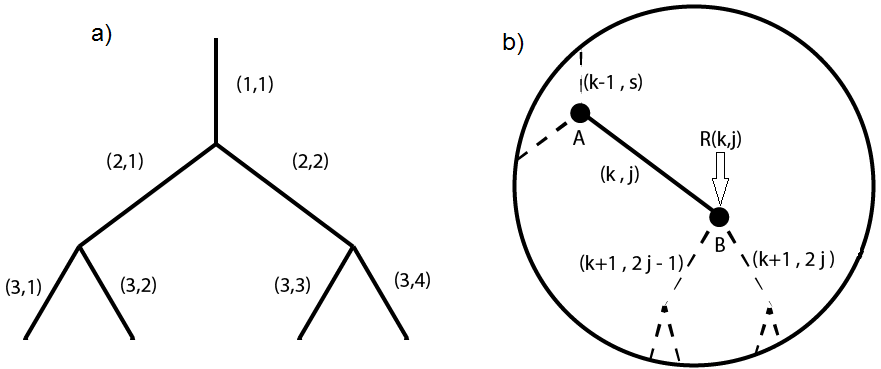
\includegraphics[scale = 0.5]{Figures/ArterialTree_Zamir.png}%
		\caption{Notação usada para identificar cada segmento de vaso $(k,j)$ (figura adaptada de~\cite{Duan}). }
		\label{fig1:arterial-tree}%
	\end{center}
\end{figure}

\subsection{Cálculo da pressão e do fluxo sanguíneo}\label{sec:pressao-fluxo}
Para determinar a pressão $\bar{p} (k,j)$ em um certo segmento $(k,j)$, aplica-se a condição de continuidade de pressão no nó proximal $A$ (ver Figura \ref{fig1:arterial-tree}). Escrevendo as componentes progressiva e atrasada da onda como $p_f (k,j)$ e $p_b (k,j)$ respectivamente, a pressão na posição proximal do segmento  $x(k,j) = 0$ é dada por:
\begin{equation}
\left[ p (k,j) \right]_A = \left[ p_f (k,j) \right]_A + \left[ p_b (k,j)\right]_A,
\label{09_p}
\end{equation}
nos quais as pressões $\left[ p_f(k,j) \right]_A$ e $\left[ p_b(k,j) \right]_A$ são expressas por:
\begin{eqnarray}
\left[ p_f(k,j) \right]_A &=& \bar{p}(k,j)\exp\left[ i\omega t\right],
\label{10_p_f}\\
\left[ p_b (k,j) \right]_A &=& R(k,j)\bar{p}(k,j)\exp\left[i\omega \left(t - \frac{2L(k,j)}{c(k,j)}\right) \right].
\label{11_p_b}
\end{eqnarray}
Similarmente, a pressão no segmento pai $(k-1,s)$ pode ser escrita como:
\begin{equation}
p(k-1,s) =  p_f(k-1,s) + p_b (k-1,s),
\label{12_p|_f}
\end{equation}
nos quais $s$ é um número sequencial do segmento pai e as pressões $ p_f (k-1,s)$ e $p_b (k-1,s)$ são dadas por:
\begin{eqnarray}
p_f (k-1,s) &=& \bar{p}(k-1,s)\exp\left[i\omega \left(t - \frac{x(k-1,s)}{c (k-1,s)}\right) \right],\\
\label{13_p_f}
p_b (k-1,s) &=& R (k-1,s)\bar{p}(k-1,s)\exp\left[ i\omega \left( t - \frac{2L(k-1,s)}{c(k-1,s)} + \frac{x(k-1,s)}{c(k-1,s)}\right) \right]. \nonumber
\end{eqnarray}

No nó distal do vaso superior, $x(k-1,s) = L(k-1,s)$, a pressão é dada por:
\begin{equation}
\left[ p(k-1,s) \right]_A = \left[ p_f(k-1,s)\right]_A + \left[ p_b(k-1,s) \right]_A,
\label{13_p|_f}
\end{equation}
nos quais 
\begin{eqnarray}
\left[ p_f(k-1,s) \right]_A &=& \bar{p}(k-1,s)\exp\left[ i\omega \left(t - \frac{L(k-1,s)}{c(k-1,s)}\right)\right],
\label{15_p_f}
\\
\left[ p_b(k-1,s) \right]_A &=& R(k-1,s)\bar{p}(k-1,s)\exp\left[i\omega \left( t - \frac{L(k-1,s)}{c(k-1,s)} \right) \right]. 
\label{16_p_b}
\end{eqnarray}

A condição de continuidade da pressão exige que na junção ela assuma um único valor, portanto
\begin{equation}
\left[ p_f(k-1,s) \right]_A + \left[ p_b (k-1,s) \right]_A = \left[ p_f(k,j) \right]_A + \left[ p_b(k,j) \right]_A.
\label{17_p_cont}
\end{equation}

Substituindo as equações \eqref{10_p_f}, \eqref{11_p_b}, \eqref{15_p_f} e \eqref{16_p_b} na equação \eqref{17_p_cont} e resolvendo para $\bar{p}(k,j)$, resulta em:
\begin{equation}
\bar{p} (k,s) =  \frac{\bar{p}(k-1,s)\left[1 + R(k-1,s)\right] \exp\left[ -\frac{i \omega L(k-1,s)}{c(k-1,s)}\right]}{1 + R(k,j)\exp{\left[ -2i\omega \frac{L(k,j)}{c(k,j)}\right]}}.
\label{18_barp}
\end{equation}

Conforme Duan e Zamir \cite{Duan}, para efeitos de cálculo da pressão e fluxo, adimensionalizam-se as pressões em \eqref{18_barp} em termos da pressão de entrada $p_0 = \bar{p}_0 \exp[i\omega t]$. 

Considerando $P(k,j) = \frac{p(k,j)}{p_0}$ e $\bar{P} (k,j) = \frac{\bar{p}(k,j)}{\bar{p}_0}$, a equação~\eqref{05_p} para o cálculo da pressão  pode ser expressa de forma adimensionalizada por:
\begin{eqnarray}
P(k,j) &=& \bar{P}(k,j)\big\{\exp[ -i\beta(k,j) X(k,j)] \nonumber \\
& +& R(k,j) \exp[-i2\beta(k,j)] \exp[i\beta(k,j) X(k,j)]\big\},
\label{21_P}
\end{eqnarray}
nos quais $\beta(k,j) = \frac{\omega L(k,j)}{c(k,j)}$ e $X = \frac{x(k,j)}{L(k,j)}$. Similarmente, a equação~\eqref{06_q} para o fluxo $q(k,j)$ pode ser obtida de forma adimensionalizada por:
\begin{eqnarray}
Q(k,j) &=& M(k,j)\bar{P}(k,j)\big\{ \exp\left[ -i\beta(k,j) X(k,j) \right] \nonumber \\ 
&-& R(k,j) \exp[ -2i\beta(k,j)] \exp[i\beta(k,j) X(k,j)] \big\},
\label{23_Q}
\end{eqnarray}
nos quais $Q(k,j) = \frac{q (k,j)}{q_0}$, $M = \frac{Y(k,j)}{Y(1,1)}$ e $q_0 = Y(1,1)p_0$. O cálculo da admitância $Y(1,1)$ na posição proximal do segmento raiz, ou seja, da artéria de alimentação é apresentado na próxima seção.

%------------------------------------------------------------%
\subsection{Cálculo dos coeficientes de reflexão e da admitância}

Para determinar os coeficientes de reflexão nas junções, consideram-se as duas junções $A$ e $B$ das extremidades de um segmento genérico $(k,j)$ de um modelo de árvore arterial (ver Figura~\ref{fig1:arterial-tree}). Na posição distal $B$, o coeficiente de reflexão é definido por~\cite{Fung,Lighthill}:
\begin{equation}
R(k,j) = \frac{Y(k,j) - [Y_e(k+1,2j) + Y_e(k+1,2j-1)]}{Y(k,j) + [Y_e(k+1,2j) + Y_e(k+1,2j-1)]},
\label{27_R}
\end{equation}
nos quais $Y_e(k+1,2j-1)$ e $Y_e(k+1,2j)$ são admitâncias efetivas nos segmentos à jusante de $B$. Estas admitâncias são determinadas pela razão entre o fluxo e pressão naquela posição, que é dada por:
\begin{equation}
Y_e(k+1,s) = \frac{Y(k+1,s)\left\{1 - R(k+1,s)\exp{[-i2\beta(k+1,s)]}\right\}}{1 + R(k+1,s)\exp{[-i2\beta(k+1,s)]}},
\label{28_Ye}
\end{equation}
nos quais $s = 2j-1$ e $2j$ são os números sequenciais dos dois segmentos filhos e $R(k+1,s)$ é o coeficiente de reflexão na posição distal de cada segmento. Similarmente, $Y_e(k,j)$, a admitância na posição proximal $A$ do segmento $(k,j)$ pode ser dada por:
\begin{equation}
Y_e(k,j) = \frac{Y(k,j)\{1 - R(k,j)\exp{[-i2\beta(k,j)]}\} }{1 + R(k,j)\exp{[-i2\beta(k,j)]}}
\label{29_Ye}.
\end{equation}
Substituindo $R(k,j)$ da equação \eqref{27_R} em \eqref{29_Ye}, obtém-se  uma equação para cálculo das admitâncias efetivas ao longo do modelo de árvore arterial:
\begin{equation}
Y_e(k,j) = \frac{Y(k,j) [Y_e(k+1,2j) + Y_e(k+1,2j-1)+ i Y(k,j)\tan{\beta(k,j)}]}{Y(k,j) + i[Y_e(k+1,2j) + Y_e(k+1,2j-1)]\tan{\beta(k,j)}}.
\label{30_Ye}
\end{equation}

Em segmentos terminais, pode ser assumido que não ocorrem mais reflexões à jusante das posições distais destes segmentos, portanto a admitância efetiva destes segmentos é igual às suas admitâncias características. Adotando a equação \eqref{29_Ye}, todas as admitâncias efetivas podem ser determinadas percorrendo a árvore a partir dos segmentos terminais até o segmento raiz.

\subsection{Cálculo da impedância de entrada}

A impedância vascular de um modelo de árvore arterial é expresso por
\begin{equation}
    z = \frac{p}{q},
\end{equation}
onde $p$ e $q$ podem ser definidos pelas equações \eqref{03_p} e \eqref{04_1}, respectivamente. Dados que $p(k,j) = P(k,j) p_0$, $q(k,j) = Q(k,j) q_0$ e $q_0 = Y(1,1) p_0$, em termos de variáveis adimensionalizadas, a impedância pode ser reescrita por
\begin{equation}
Z = \frac{P(k,j)}{Y(1,1) Q(k,j)}.
\end{equation}

A impedância de entrada de um modelo de árvore arterial determina $Z$ na posição proximal do vaso raiz, ou seja, em $x (k,j) = 0$. 

Adotando as equações~\eqref{21_P} e~\eqref{23_Q} com $x (k,j) = 0$, obtém-se a impedância de entrada:
\begin{equation}
Z = \frac{-1}{Y(1,1)}.
\end{equation}
Em suma, a impedância de entrada  em módulo é o inverso da admitância característica da artéria de alimentação.

%--------------------------------------------------------------------------------%
\subsection{Incorporação da viscosidade e viscoelasticidade no modelo}
\label{sec:cenario}
A partir do modelo matemático aqui apresentado, os seguintes cenários podem ser investigados nas simulações hemodinâmicas:
\begin{itemize}
	\item \textbf{cenário 1}: análise do impacto da viscosidade sanguínea ($\mu(k,j)$).\\
	Os efeitos da viscosidade sanguínea podem ser investigados por substituir a velocidade
	da onda $c(k,j)$ por uma velocidade da onda complexa~\cite{Duan1992}:
	\begin{equation} 
	c_v(k,j) = c(k,j) \sqrt{\epsilon},\label{eq:velocidade-complexa}
	\end{equation}
	onde $\epsilon$ é um fator viscoso que corresponde a um tubo elástico com restrições~\cite{Duan1992}. Seja $\alpha$ o
	número de Womersley adimensional
	\begin{equation}
	\alpha = r(k,j) \sqrt{\frac{\omega \rho(k,j)}{\mu(k,j)}},
	\end{equation}
	o fator viscoso $\epsilon$ é calculado por:
	\begin{equation}
	\epsilon = 1 - F_{10} (\alpha),
	\end{equation}
	onde a função $F_{10}$ é avaliada deste modo:
	\begin{equation}
	F_{10} (\alpha) = \frac{2 J_1(i^{1,5} \alpha)}{\alpha i^{1,5}J_0(i^{1,5} \alpha)},
	\end{equation}
	onde $J_p$ denota a função de Bessel de índice $p$.
	
	\item \textbf{cenário 2}: análise do impacto da viscoelasticidade da parede do vaso ($\phi_0$).\\
	A viscoelasticidade da parede do segmento é incorporado substituindo o módulo de Young
	estático $E(k,j)$ por um módulo elástico complexo $E_c(k,j)$ no cálculo da velocidade $c(k,j)$ na equação~\eqref{eq:velocidade}
	da seguinte forma~\cite{Duan}:
	\begin{equation}
	E_c(k,j) = |E_c(k,j)| \exp\{i\phi\},\label{eq:Young}
	\end{equation}
	onde $\phi$ é o ângulo de fase entre a pressão e o deslocamento da parede do segmento \cite{Taylor3} expresso por $\phi = \phi_0 [1-\exp(-\omega)]$ e $|E_c (k,j)|$ corresponde ao módulo de Young fornecido para a simulação.
	
	\item \textbf{cenário 3}: efeitos da viscosidade sanguínea ($\mu(k,j)$) e da viscoelasticidade da parede do segmento ($\phi_0$) de forma combinada.
	
	Neste último cenário, utiliza-se a equação~\eqref{eq:Young} para determinar a velocidade da onda $c(k,j)$~\eqref{eq:velocidade} no modelo. Com este resultado, calcula-se  a equação~\eqref{eq:velocidade-complexa} para determinar a velocidade complexa $c_v(k,j)$ a ser considerada no modelo.
\end{itemize}

\section{MODELAGEM COMPUTACIONAL}
\label{sec:algoritmo}
Nesta seção, detalham-se alguns aspectos da estrutura de dados e algoritmos que descrevem os passos para o cálculo das ondas de pressão $P(j,k)$ e fluxo $Q(j,k)$.

Inicialmente, salientam-se que as equações~\eqref{27_R} e~\eqref{28_Ye} expõem a necessidade de valores $Y_e(k+1,2j)$ e $Y_e(k+1,2j-1)$ atrelados às artérias adjacentes na posição distal do segmento $(k,j)$. Por outro lado, o valor da pressão média do segmento $(k,j)$ calculado usando a equação~\eqref{18_barp} depende de valores  à montante desse segmento, ou seja, do valor $\bar{p}(k-1,s)$. Tendo isto em vista, a estrutura de dados desenvolvida utiliza de ponteiros para acessar as propriedades de artérias à montante e a jusante de um vaso do modelo.

Neste trabalho, adotou-se a linguagem de programação C++. Essa linguagem de programação escolhida permite que objetos \textcolor{red}{sejam passados por referência. Ao passar um objeto por referência, o endereço de memória é enviado, dando total acesso aos parâmetros do objeto, este endereço é chamado de ponteiro. Ao enviar o ponteiro do segmento raiz, é possível acessar todo o modelo de árvore arterial}. Cada vaso arterial do modelo contém as propriedades apresentadas na Tabela~\ref{tab:info_vaso}, além de ponteiros para os vasos adjacentes. 

\begin{table}[h]
\begin{tabular}{|c|c||c|c|}
	\hline
	\textbf{valores conhecidos} & \textbf{unidade} & \textbf{valores calculados} & \textbf{unidade} \\
	\hline
	comprimento ($L$) & cm &  velocidade da onda ($c$) & cm/s \\
	
	densidade ($\rho$) & g/cm$^3$ &   beta ($\beta$) & -- \\

	 módulo de Young ($E$) & g/cms$^2$  & velocidade angular ($\omega$) & rad/s \\
	 
 viscosidade ($\mu_0$) & cm$^2$/s &	espessura da parede ($h$) &  cm \\

	raio ($r$) & cm  & número de Womersley ($\alpha$) & --- \\
	
	 & & admitância característica ($Y$) & $cm^4 s/g $\\
	
 &  & admitância efetiva ($Y_e$) & $cm^4 s/g $\\
	
	&  & coeficiente de reflexão ($R$) & $g /cm^4 s$ \\
		
	& & fator viscoso ($\epsilon$) & --- \\
	
& & pressão ($P$) & -- \\
	
  &  &	pressão média ($\bar{p}$) & --- \\
  	
 & &	fluxo ($Q$) & -- \\
\hline
\end{tabular}
\caption{Propriedades de cada vaso arterial do modelo.}
\label{tab:info_vaso}
\end{table}

Além das propriedades especificadas na Tabela~\ref{tab:info_vaso}, o vaso possui ainda três ponteiros para os seus vasos adjacentes. Um destes ponteiros, para o vaso adjacente ao seu nó proximal, ou seja, para o seu vaso pai $(k-1,s)$. Os demais ponteiros para os vasos adjacentes ao seu nó distal, ou seja, para seus vasos filhos à esquerda e à direita expressos por $(k+1,2j-1)$ e $(k+1,2j)$, respectivamente. Este arranjo de ponteiros é equivalente a uma árvore duplamente encadeada, onde através de um único ponteiro para um vaso é possível trafegar a árvore nos dois sentidos. Isto é útil quando é necessário acessar propriedades de outro vaso para se determinarem por exemplo, a pressão média, coeficientes de reflexão e admitâncias de um dado vaso.

Os ponteiros permitem também definir se o vaso é a raiz ou uma folha. Caso o ponteiro para o segmento superior $(k-1,s)$ seja igual ao valor da \textit{flag} nula se trata de um vaso raiz. Caso ambos vasos  $(k+1,2j-1)$ e $(k+1,2j)$ sejam iguais ao valor da \textit{flag} nulo se trata de vaso folha, isto é, um vaso terminal.

Basicamente, os passos para determinar as ondas de pressão e fluxo que percorrem um modelo de árvore arterial usando o modelo de Duan e Zamir são dados por:
\begin{enumerate}
    \item Cálculo da admitância característica $(Y)$ de cada segmento;
    \item Cálculo da admitância efetiva $(Y_e)$  de cada segmento;
    \item Cálculo do coeficiente de reflexão $(R)$  de cada segmento; 
    \item Armazenar valor da admitância característica $(Y_r)$ do segmento raiz;
    \item Cálculo da pressão média $(\bar{p})$ em cada segmento;
    \item Cálculo das ondas de pressão e fluxo $P$ e $Q$.
\end{enumerate}

Os passos acima mencionados podem ser organizados no Algoritmo 1. Esse algoritmo tem como entrada: o modelo de árvore arterial ($\mathcal{MAA}$) com seus vasos caracterizados por suas propriedades, a frequência ($f$) em Hz, um fator de escala da viscosidade ($\gamma_{\mu}$), e o parâmetro da viscoelasticidade da parede ($\phi$). 

O Algoritmo 1 proposto tem dois módulos. O primeiro módulo realiza o cálculo percorrendo o caminho a partir dos vasos finais até o vaso raiz (estratégia do tipo \textit{bottom-up}). O segundo módulo realiza cálculos percorrendo o modelo a partir do vaso raiz até os vasos terminais (abordagem do tipo \textit{top-bottom}).

\begin{algorithm}[H]
	\SetAlgoLined
	\Entrada{ $\mathcal{MAA}$, $f$, $\gamma_{\mu}$, $\phi$, $\bar{p}_0$ }
	\Inicio{
		inicializa vaso $s$ a partir do vaso raiz;\\
		\Se{existe($s$)}{
			Chama $\mathcal{M}_1$ ($s$, $f$, $\gamma_{\mu}$, $\phi_0$) e armazena $Y_r$
		}
		\Se{existe($Y_r$)}{
			Chama $\mathcal{M}_2$($s$ , $\bar{p}_0$, $Y_r$);
		}
	}
\caption{Cálculos hemodinâmicos do modelo de árvore arterial ($\mathcal{MAA}$).}
\end{algorithm}

Antes que algum módulo possa ser executado é necessário que o ponteiro recebido pelo algoritmo representa de fato uma vaso arterial

O módulo $\mathcal{M}_1$ do Algoritmo 1  visa calcular os valores de admitância efetiva ($Y_e$), admitância característica ($Y$) e coeficiente de reflexão ($R$) de cada vaso. Desta forma, é necessário que as admitâncias efetivas dos vasos à justante do segmento $k$ ($Y_e(k+1,2j-1)$ e $Y_e(k+1,2j)$) já estejam definidas. Em vista disso, verifica-se a existência dos vasos à justante do vaso atual tanto a esquerda ($esq$) quanto a direita ($dir$) e caso existam realiza-se uma chamada recursiva. Após o retorno das chamadas recursivas calculam-se as propriedades do vaso atual. Assim, as propriedades do vasos à jusante do vaso atual serão conhecidas, ou seja, já terão sido determinadas $Y_e(k+1,2j-1)$ e $Y_e(k+1,2j)$.

\begin{algorithm}[H]
$\mathcal{M}_1$ ($s$, $f$, $\gamma_{\mu}$, $\phi_0$) \\
	\Inicio{
		\Se{existe($s \rightarrow esq$)}{
			$\mathcal{M}_1$ ($s \rightarrow esq$, $f$, $\gamma_{\mu}$, $\phi_0$);
		}
		\Se{existe($s \rightarrow dir$)}{
			$\mathcal{M}_1$ ($s \rightarrow dir$, $f$, $\gamma_{\mu}$, $\phi_0$);
		}
		Calcula as propriedades $c$, $\omega$, $\beta$; \\
		\Se{ ($\gamma_{\mu} == 0$ e $\phi == 0$) }{
			Calcula $Y$;
		}
		\Senao{
		    \Se{ ($\gamma_{\mu} != 0$) }{
			Calcula $\alpha$, $\epsilon$, $E_v$, $c_v$ e $Y_v$;\\
			Atualize $E = E_v$, $c = c_v$ e $Y = Y_v$;
			}
		    \Se{ ($\phi != 0$) }{
			Calcula $E_c$;\\
			Atualize $E = E_c$;
			}
		}
		\Se{(s é um vaso terminal)}{
			$Y_e = Y$ e  $R = 0$;
		}
		\Senao{
			Calcula $Y_e$ e $R$;
		}
	}
	\caption{$\mathcal{M}_1$ -- Cálculo das admitâncias e coeficiente de reflexão.}
\end{algorithm}

\textcolor{red}{PAREI AQUI}
O módulo 2 do Algoritmo 1 visa calcular o valor da pressão média, pressão e fluxo em cada vaso. Como expresso na equação~\eqref{18_barp}, o valor da pressão média requer o valor da pressão média do vaso à montante $(k-1,s)$. Com isso, verifica-se, inicialmente, se o vaso atual é a artéria de alimentação (raiz), neste caso $\bar{p} = \bar{p}_0$. Caso contrário, calcula-se $\bar{p}$ com a equação~\eqref{18_barp}. Em seguida, o valor das ondas de pressão e fluxo são obtidas ao longo de cada vaso 1D, que são discretizados. Por fim, a recursão é enviada aos segmentos inferiores, desta forma se garante a existência de um valor $\bar{p}(k-1,s)$.

\begin{algorithm}[H]
\textbf{\textit{\textsl{\underline{fase dois}}}}(a,f,$\epsilon$,$\phi_0$) \\
\Inicio{
	\Se{a $\in$ raiz}{
		$\bar{p} = \bar{p_0}$
	}
	\Senao{
		Calcula $\bar{p}$
	}
	Calcula $P(X) e Q(X) \forall X \in [0,1])$ \\
	\Se{existe(a $\rightarrow$ esquerda)}{
		Envia a recursão \textit{fase dois}(a $\rightarrow$ esquerda,f,$\epsilon$,$\phi_0$)
	}
	\Se{existe(a $\rightarrow$ direita)}{
		Envia a recursão \textit{fase dois}(a $\rightarrow$ direita,f,$\epsilon$,$\phi_0$)
	}
}
\caption{Segunda fase do cálculo, recursão \textit{(bottom-up)}.}
\end{algorithm}

Ao término da execução os valores contidos na artéria são analisados separadamente. A onda de pressão e fluxo representa um conjunto de valores por segmento que precisam ser calculados e armazenados, para isto é preciso determinar a quantidade de pontos $N$ que serão analisados dentro do espaço $X \in [0,1]$, foi adotado $N = 101$. No caso da onda de pressão os valores encontrados para ramo de árvore deve resultar em um gráfico contínuo, isto é $P(k,j)(X=0) = P(k+1,2j)(X=1)$ e $P(k,j)(X=0) = P(k+1,2j-1)(X=1)$.
	
%--------------------------------------------------------------------------------%
\chapter{Ferramenta computacional}\label{sec:modelagem}

Nesta seção apresentam-se detalhes da ferramenta computacional desenvolvida para simulação do escoamento sanguíneo em modelos de árvores arteriais. Com esta ferramenta, o usuário poderá  visualizar a estrutura da árvore arterial e depois da simulação hemodinâmica, visualizar curvas de distribuição de fluxo sanguíneo e pressão.

Esta ferramenta foi desenvolvida em C++ utilizando as bibliotecas comuns do Qt 5.15.0 \cite{QTClasses} e do OpenGL \cite{OpenGL}, que ajudam na construção da interface gráfica e na exibição de objetos, como árvores arteriais e gráficos. Ela foi nomeada de \textit{Iterador Gráfico Universal} (IGU), pois em seu modelo de classes qualquer objeto que implemente a classe \textit{WiseObject}, elucidada na Seção~\ref{sec:estrutura}, está apto para realizar iterações e desenhar-se através de diretivas OpenGL em um objeto de interface gráfica. Buscou-se no desenvolvimento desta ferramenta alto grau de generalização para que possa ser utilizada por diferentes objetos dentro do ambiente. Além de árvores arteriais menciona-se que a ferramenta itera diferentes estruturas de dados, entre eles malhas estruturadas e não estruturadas, por isto uma nomenclatura genérica.

A Figura~\ref{fig1:gui} ilustra a ferramenta desenvolvida. À seguir, apresentam-se em detalhes a implementação computacional realizada.

\begin{figure}[!htbp]
	\centering
	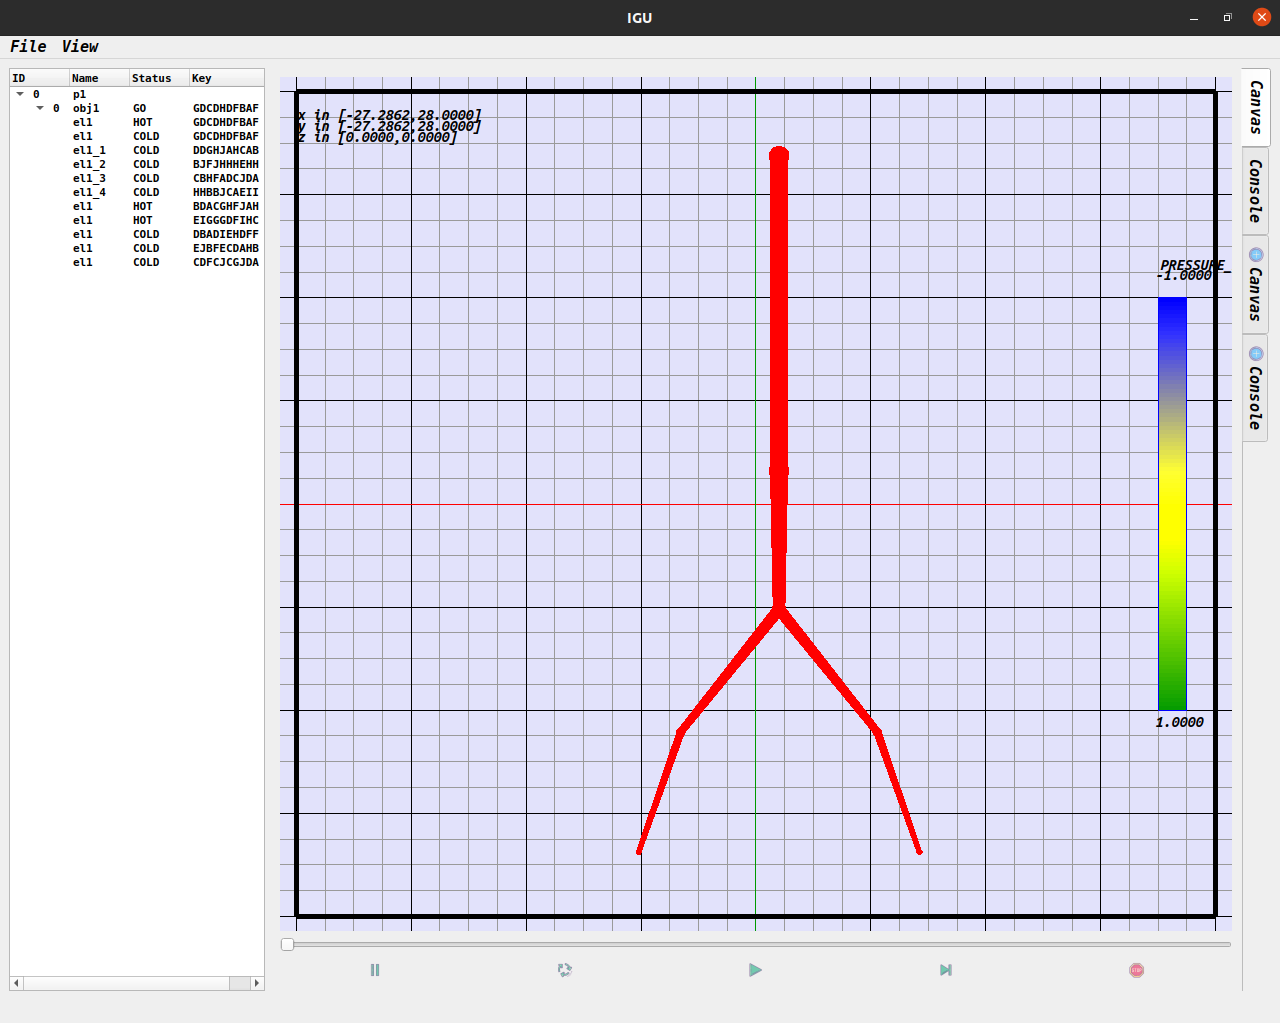
\includegraphics[scale=0.25]{Figures/IGU.png}
	\caption{Interface gráfica da ferramenta desenvolvida.}
	\label{fig1:gui}
\end{figure}

Através da modelagem de classes no paradigma do C++ \cite{AlanParker}, foi possível realizar diversas generalizações para ampliar a quantidade de objetos que podem ser inseridos neste modelo de classes. Na seção seguinte apresentamos um esquema de classes virtuais, ou abstratas, que foram criadas para facilitar o manuseio dos objetos dentro do ambiente computacional e prover funções básicas, a classe \textit{WiseElement}. Objetos que recebem essa estrutura básica por herança são nomeados de elementos inteligentes.

%--------------------------------------------------------------------------------%
\section{Estrutura de Dados}\label{sec:estrutura}

Nesta seção apresentam-se detalhes da estrutura de dados adotada no funcionamento da ferramenta computacional. Como mencionado na Seção~\ref{sec:algoritmo} é utilizada uma estrutura de ponteiros que é capaz de armazenar todas as informações do modelo geométrico da árvore arterial. A ferramenta computacional foi desenvolvida para ser capaz de armazenar, carregar e iterar este modelo bem como gerar novas estruturas para visualização.

As seções à seguir descrevem a estrutura de dados genérica, sendo o modelo principal de estudo é o estudo do fluxo pulsátil atravessando a estrutura de uma árvore arterial e a visualização de seus resultados. Em versões anteriores deste ambiente computacional os objetos eram definidos em apenas uma classe abstrata, com diversos métodos virtuais que precisavam ser implementados, isto acarretava em lasses herdeiras extremamente complexas. Isto porque o mesmo objeto ficava responsável por mais de uma função, era capaz de se instanciar, de se iterar e se desenhar na tela através de diretivas OpenGL. Além disso, após iterar o objeto repetidas vezes não era possível analisas objetos de iterações passadas, isto porque os dados eram sempre sobrescritos.

Com estas barreiras em mente, a classe representante do modelo foi dividida em suas funções e fábricas ficam responsáveis por suas novas instâncias. A classe de elemento inteligente, \textit{WiseElement}, que é responsável por manter uma estrutura genérica  do modelo e gerenciar a localização desta estrutura. Outra atribuição dada as fábricas foi a iteração dos modelos contidos em um elemento inteligente, isto porque o processo de iteração envolve a criação de um novo objeto para que não haja sobrescrita. Os objetos gráficos, \textit{GraphicObject}, são objetos criados à partir da estrutura contida em um elemento inteligente que são capazes de se desenhar.

%--------------------------------------------------------------------------------%
\subsection{Elemento Inteligente}\label{sec:elemento_inteligente}

Através das estruturas estruturadas e desestruturadas presentes na biblioteca \textit{VTK}(\textit{Visualization ToolKit}) é posível descrever os mais diversos tipos de dados com diretivas simples. Baseando-se nessa estrutura básica a arquitetura presente na Figura~\ref{fig2:wiselement} foi criada.

\begin{figure}[!htbp]
	\centering
	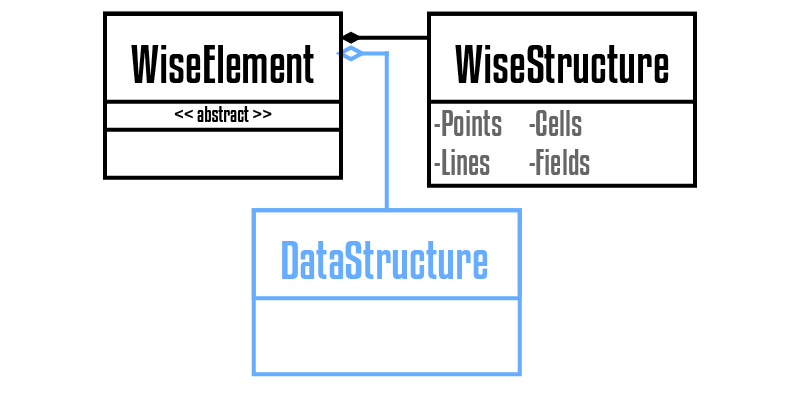
\includegraphics[scale=1]{Figures/WiseElement.png}
	\caption{Representação de classes de um elemento inteligente. WiseElement a classe abstrata base e seus componentes: WiseStructure representa a estrutura contida em um arquivo VTK e DataStructure representa a estrutura de ponteiros e variáveis utilizadas na iteração. Tingido de azul as estruturas que nem sempre estão presentes.}
	\label{fig2:wiselement}
\end{figure}

A Figura~\ref{fig2:wiselement} mostra que um elemento inteligente é composto por duas outras estruturas: A primeira \textit{WiseStructure}, utiliza pontos, linhas, células e campos para determinar estruturas geométricas; A segunda \textit{DataSructure}, representa os dados abstratos específicos de cada elemento. Estas estruturas são equivalentes entre si, isto é feito para que a estrutura siga um formato padrão de pontos, linhas, células e campos seja mantida enquanto dados abstratos equivalentes podem ser utilizados. Isto significa que os dados de uma árvore arterial estão disponíveis na estrutura padrão \textit{WiseStructure} e também disponibiliza ponteiros através da \textit{DataStructure} de uma \textit{WiseArteryTree}.

\begin{figure}[!htbp]
	\centering
	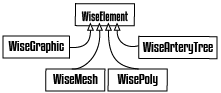
\includegraphics[scale=1]{Figures/WiseElements.png}
	\caption{Tipos de elementos inteligentes. \textit{WiseGraphic}, um gráfico bidimensional. \textit{WiseMesh}, uma malha bidimensional. \textit{WisePoly}, uma malha tridimensional. \textit{WiseArteryTree}, uma árvore arterial}
	\label{fig2:wiselements}
\end{figure}

 Como demonstrado na Figura~\ref{fig2:wiselements} um elemento inteligente é aquele que implementa a classe abstrata \textit{WiseElement}, os dados abstratos de cada classe podem ser salvos na estrutura disponível (\textit{WiseStructure}) e utilizados quando necessário. 
 
 Os elementos inteligentes servem como estruturas de armazenamento padrão para que possam ser utilizados por outros objetos. O ciclo de manipulação desses elementos se divide em três partes: A criação, aonde os objetos podem ser criados à partir de exemplos pré-definidos ou através de um arquivo de entrada \textit{VTK} ou \textit{XML (eXtensible Markup Language)}; A iteração, processo em que o elemento inteligente com todas as estruturas definidas e consistentes é utilizado para o cálculo de alguma lógica pré-definida; A exibição,  como os elementos inteligentes possuem uma variedade de parâmetros, foi criada uma estrutura com um único parâmetro que é especializada em desenhar-se na tela.
 
O elemento inteligente então poderá ser representado em qualquer uma das estruturas que o compõe, sendo \textit{DataStructure} a estrutura de dados abstratos utilizados em cada iteração e a \textit{WiseStructure} utilizada principalmente para leitura e escrita. Em seguida, poderá ser também visualizado ao criar-se uma estrutura equivalente \textit{GraphicObject}, que possuirá os elementos gráficos e as diretivas \textit{OpenGL} necessárias para visualizar a forma.

\begin{figure}[!htbp]
	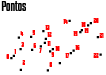
\includegraphics[width=0.33\textwidth]{Figures/WiseElementPoints.png}
	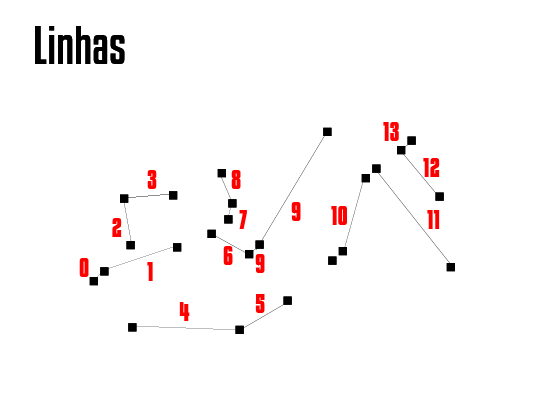
\includegraphics[width=0.32\textwidth]{Figures/WiseElementLines.png}
	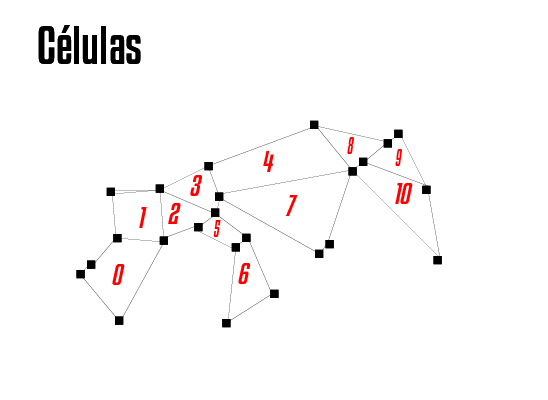
\includegraphics[width=0.33\textwidth]{Figures/WiseElementCells.png}
	\caption{Pontos utilizados na especificação do modelo geométrico. Linhas utilizadas na especificação do modelo geométrico, através dos pontos previamente definidos. Células utilizadas na especificação do modelo geométrico, através dos pontos previamente definidos.}
	\label{fig2:wiselementstructs}
\end{figure}

Utilizando pontos e linhas é possível representar o mesmo modelo geométrico de uma árvore arterial, basta considerar cada ponto uma bifurcação de vasos e cada segmento de vaso uma linha. Através dessa estrutura de dados é possível armazenar e acessar dados sobre cada ponto e linha, desta forma é possível armazenar as informações de cada segmento pertencente à uma árvore arterial através da estrutura \textit{WiseStructure}. Para dados gerais do modelo, como a frequência $f$, os campos da estrutura são utilizados.

Isto foi feito para facilitar a leitura e escrita de objetos, pois a classe \textit{WiseElement} foi desenvolvida para construir a estrutura abstrata (\textit{DataStructure}) à partir das informações contidas na estrutura inteligente (\textit{WiseStructure}). A estrutura abstrata não está sempre presente, pois como veremos é custoso manter em memória esta estrutura para todos os elementos. Portanto, todos os elementos inteligente obedecem à máquina de status contida na Figura~\ref{fig3:wiselementstatus}.

\begin{figure}[!htbp]
	\centering
	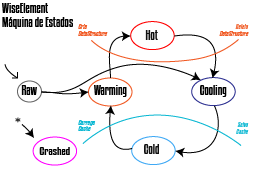
\includegraphics[scale=1.5]{Figures/WiseElementStatus.png}
	\caption{Máquina de Status que controla o funcionamento de um elemento inteligente.}
	\label{fig3:wiselementstatus}
\end{figure}

Todo elemento inteligente é criado no estado \textit{Raw}, ou cru, que representa um elemento ainda sem estruturas carregadas. Uma vez que a estrutura inteligente é inserida e verificada o elemento muda para o status \textit{Warming} ou \textit{Cooling}, respectivamente esquentando ou esfriando, que estão representados na Figura~\ref{fig4:wiselementwarming}.

\begin{figure}[!htbp]
	\centering
	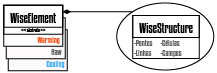
\includegraphics[scale=1]{Figures/WiseElementWarming.png}
	\caption{Elemento inteligente enquanto no estado \textit{Warming}.}
	\label{fig4:wiselementwarming}
\end{figure}

A estrutura contida em um elemento no estado \textit{Warming} é igual à dos estados \textit{Raw} e \textit{Cooling}. Os estados diferem em finalidade, enquanto o estado \textit{Warming} indica que o elemento está esperando a construção de sua estrutura abstrata (\textit{DataStructure}). O estado \textit{Raw} indica que não é esperado que os dados sejam consistentes e o estado \textit{Cooling} indica que o elemento aguarda que seus dados sejam salvos em cache.

Como demonstrado na figura~\ref{fig3:wiselementstatus}, o estado frio (\textit{Cold}) está associado com o uso de um cache para elementos estruturais, onde somente a estrutura \textit{WiseStructure} é salva. A estrutura representa um arquivo VTK mas são efetivamente salvos em um arquivo \textit{XML}. Caso sejam novamente carregados por uma mudança de estado ou deletados o arquivo em cache é deletado. Quando um elemento inteligente está neste estado ele contém apenas o endereço para o arquivo em que foi armazenado.

\begin{figure}[!htbp]
	\centering
	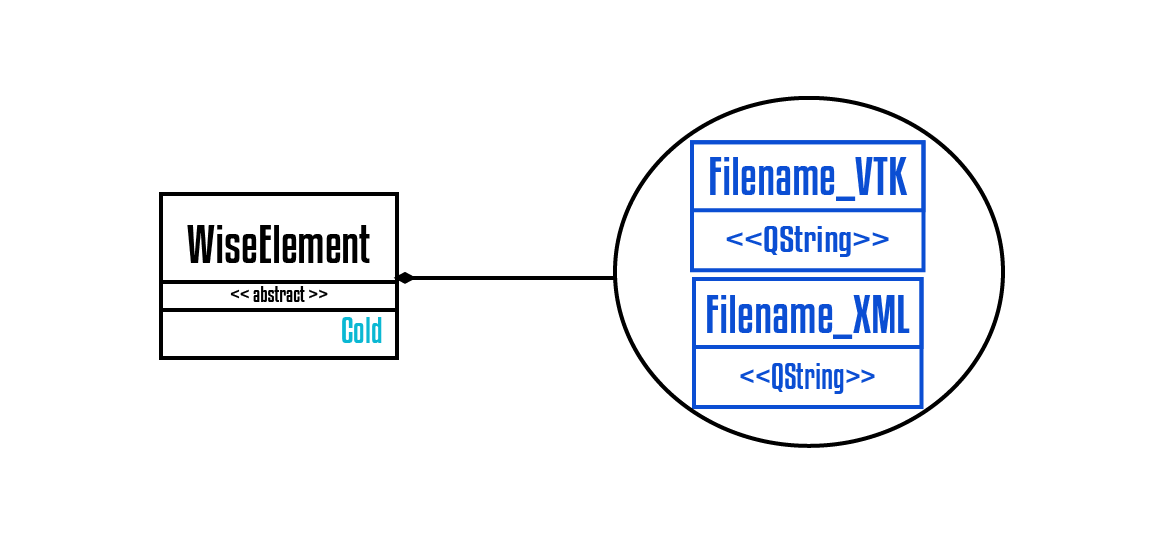
\includegraphics[scale=1]{Figures/WiseElementCold.png}
	\caption{Elemento inteligente enquanto no estado \textit{Cold}.}
	\label{fig5:wiselementcold}
\end{figure}

O estado \textit{Crashed} serve para identificar objetos que não tem mais o funcionamento esperado. Durante a troca de estados do elemento é sempre verificado se os elementos esperados estão presentes, caso não estejam o objeto fica com este estado.

Finalmente, o estado \textit{Hot} representa os elementos que possuem todas as estruturas presentes. No caso de uma árvore arterial \textit{WiseArteryTree} isto significa que a estrutura geométrica da \textit{WiseStructure} está carregada e a estrutura abstrata equivalente \textit{DataStructure} está presente e consistente.

\begin{figure}[!htbp]
	\centering
	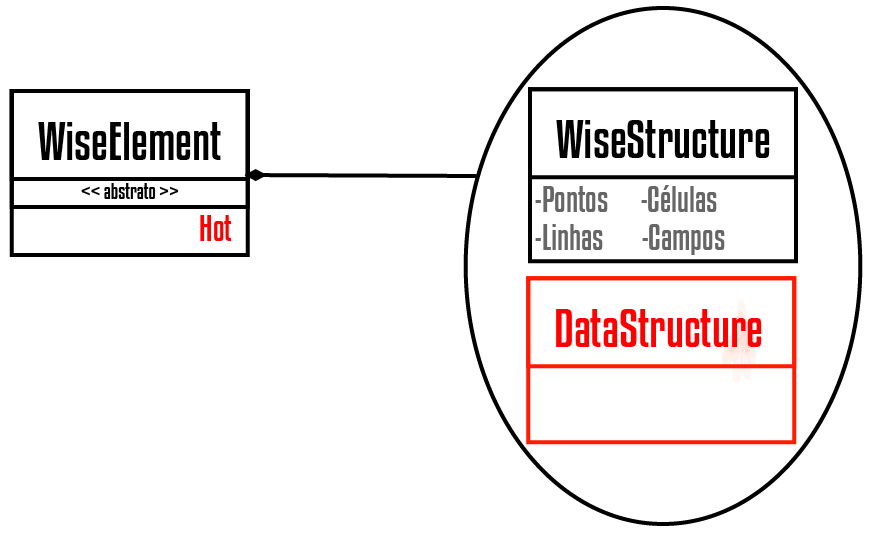
\includegraphics[scale=1]{Figures/WiseElementHot.png}
	\caption{Elemento inteligente enquanto no estado \textit{Hot}.}
	\label{fig6:wiseelementhot}
\end{figure}

Para que um elemento possa ser iterado por alguma fábrica do tipo \textit{WiseIterationFactory} ele precisa estar no estado \textit{Hot}, isto porque durante a iteração os dados abstratos são utilizados. A cada passo da iteração a estrutura \textit{DataStructure} é atualizada, exigindo uma atualização da estrutura \textit{WiseStructure}. Apenas a estrutura de um elemento inteligente não é capaz de armazenar todos os passos da iteração, isto é, a cada atualização os dados são sobrescritos.

%--------------------------------------------------------------------------------%
\subsection{Fábricas}\label{sec:fabricas} 
 
Com estes passos em mente foi idealizada uma arquitetura de classes que permite a execução de cada passo através do paradigma de Fábricas Dinâmicas~ \cite{factorypattern}. Uma arquitetura com fábricas permite a criação de instâncias com definições concretas, armazenadas como metadados. Isso facilita a adição de novos objetos que podem ser interpretados sem modificar o código da fábrica em si.

\begin{figure}[!htbp]
	\centering
	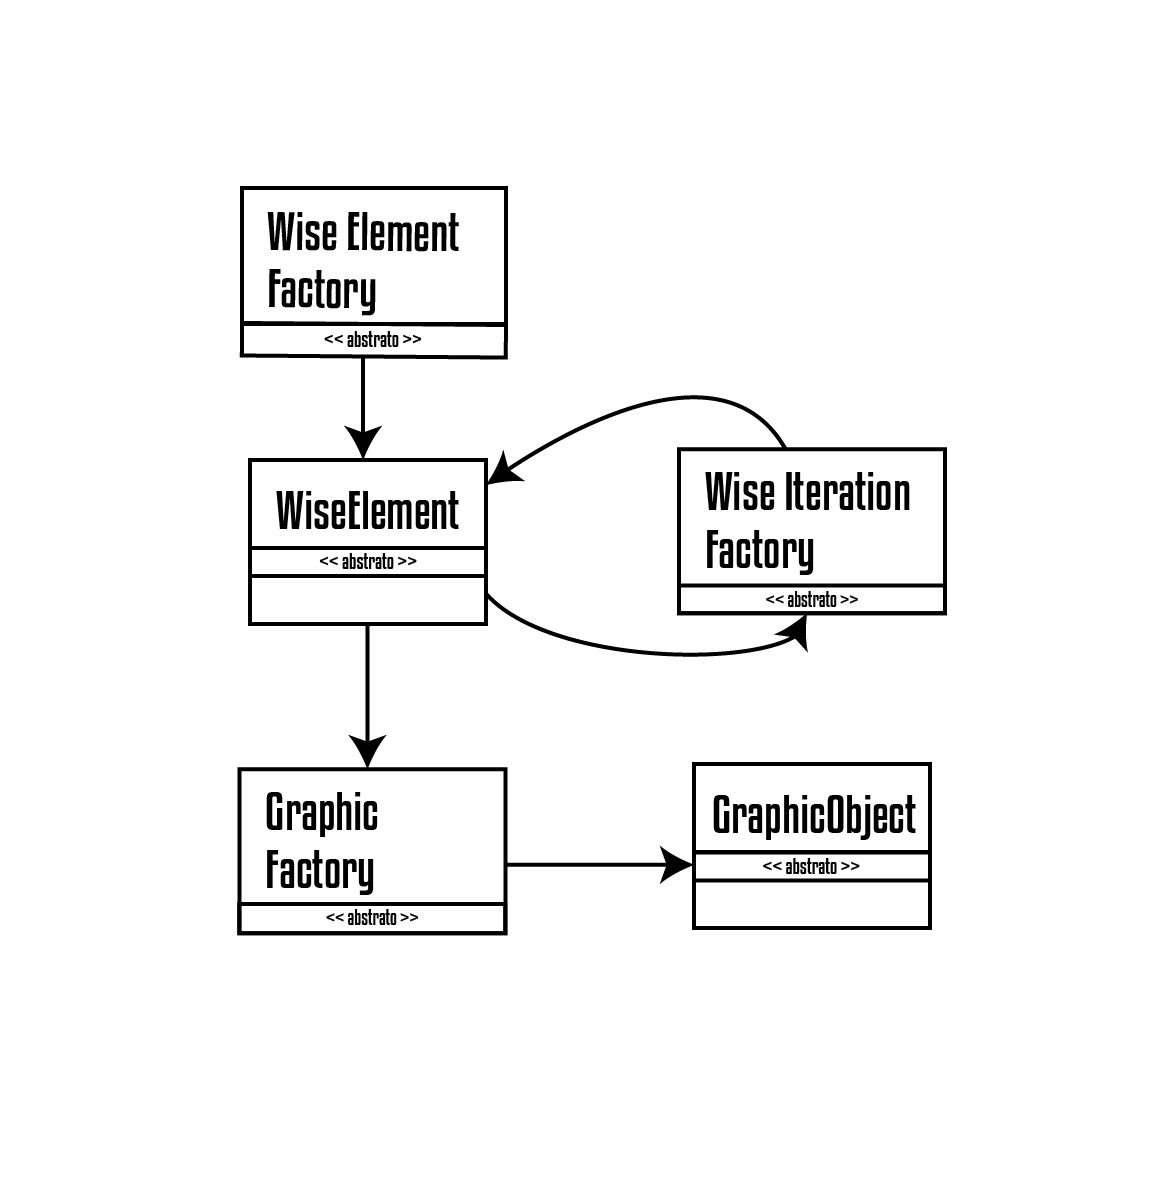
\includegraphics[scale=1]{Figures/WiseElementWorkflow.png}
	\caption{Arquitetura de classes fábrica e fluxo de trabalho do elemento inteligente WiseElement. A fábrica WiseElementFactory é responsável por criar o elementos inteligentes, a fábrica WiseIterationFactory é reponsável pela iteração do elemento inteligente e a fábrica GraphicFactory é responsável por criar as estrturas de visualização. }
	\label{fig2:wiselementsworkflow}
\end{figure}
 
Primeiramente, a fábrica \textit{WiseElementFactory}  é utilizada para a criação de elementos inteligentes, ao se criar um elemento à partir de um exemplo é preciso identificar o tipo de objeto à ser criado e qual exemplo será utilizado. Caso seja um arquivo \textit{VTK} é necessário informar apenas o tipo e caminho do arquivo. Com um arquivo \textit{XML} só o caminho do arquivo é necessário, pois a fábrica ao ler o XML identifica o tipo de elemento inteligente e identifica qual fábrica é a responsável por recriar aquele tipo de objeto. Devido à forma como os dados são carregados para cada elemento, é necessário que haja uma fábrica para cada tipo de elemento inteligente.

A fábrica \textit{WiseIterationFactory} também só pode operar com um tipo específico de elemento inteligente, entretanto é possível que haja mais de uma fábrica de iteração disponível por tipo de elemento inteligente. Desta forma uma árvore arterial pode ser iterada por diferente algoritmos de iteração e o mesmo ocorre com os outros tipos de elementos. Estas fábricas são responsáveis por executar algum algoritmo que utilize o tipo de dados do elemento inteligente. No caso de uma árvore arterial é possível utilizar uma fábrica que irá executar o modelo matemático descrito na seção~\ref{sec:algoritmo} utilizando os ponteiros para segmentos disponíveis em uma \textit{WiseArteryTree}.

Por último, a fábrica \textit{GraphicFactory} irá criar o objeto gráfico correspondente ao elemento inteligente. Assim como um elemento inteligente um objeto gráfico pode ser salvo em cache, contudo somente em um arquivo \textit{XML}.  Um elemento inteligente é composto por todas as linhas, pontos, células e seus valores associados, enquanto um objeto gráfico contém todos os elementos gráficos, como esferas, pontos e outros elementos gráficos, entretanto armazena apenas um valor associado à cada elemento gráfico. O que significa que só é possível selecionar um parâmetro por vez ao visualizar um objeto gráfico.


%--------------------------------------------------------------------------------%
\subsection{Objeto Inteligente}\label{sec:objeto_inteligente}

Para preservar todos os passos de de iteração e poupar a quantidade de recursos mantida em memória, a classe \textit{WiseObject}, ou objeto inteligente foi idealizada. Um objeto inteligente é composto por um coleção de elementos inteligentes e objetos gráficos equivalentes entre si. Neste tipo de objeto é facultativa a presença de uma fábrica gráfica, possibilitando que objetos sejam iterados sem que alguma estrutua seja disponibilizada para visualização. Foi utilizada novamente uma arquitetura de fábricas para garantir que um objeto inteligente seja criado corretamente, pode-se criar um objeto inteligente através de um elemento inteligente previamente definido, este elemento será clonado e uma instância será aquecida na estrutura \textit{Forno} enquanto a outra será congelada na estrutura \textit{Freezer}.

\begin{figure}[!htbp]
	\centering
	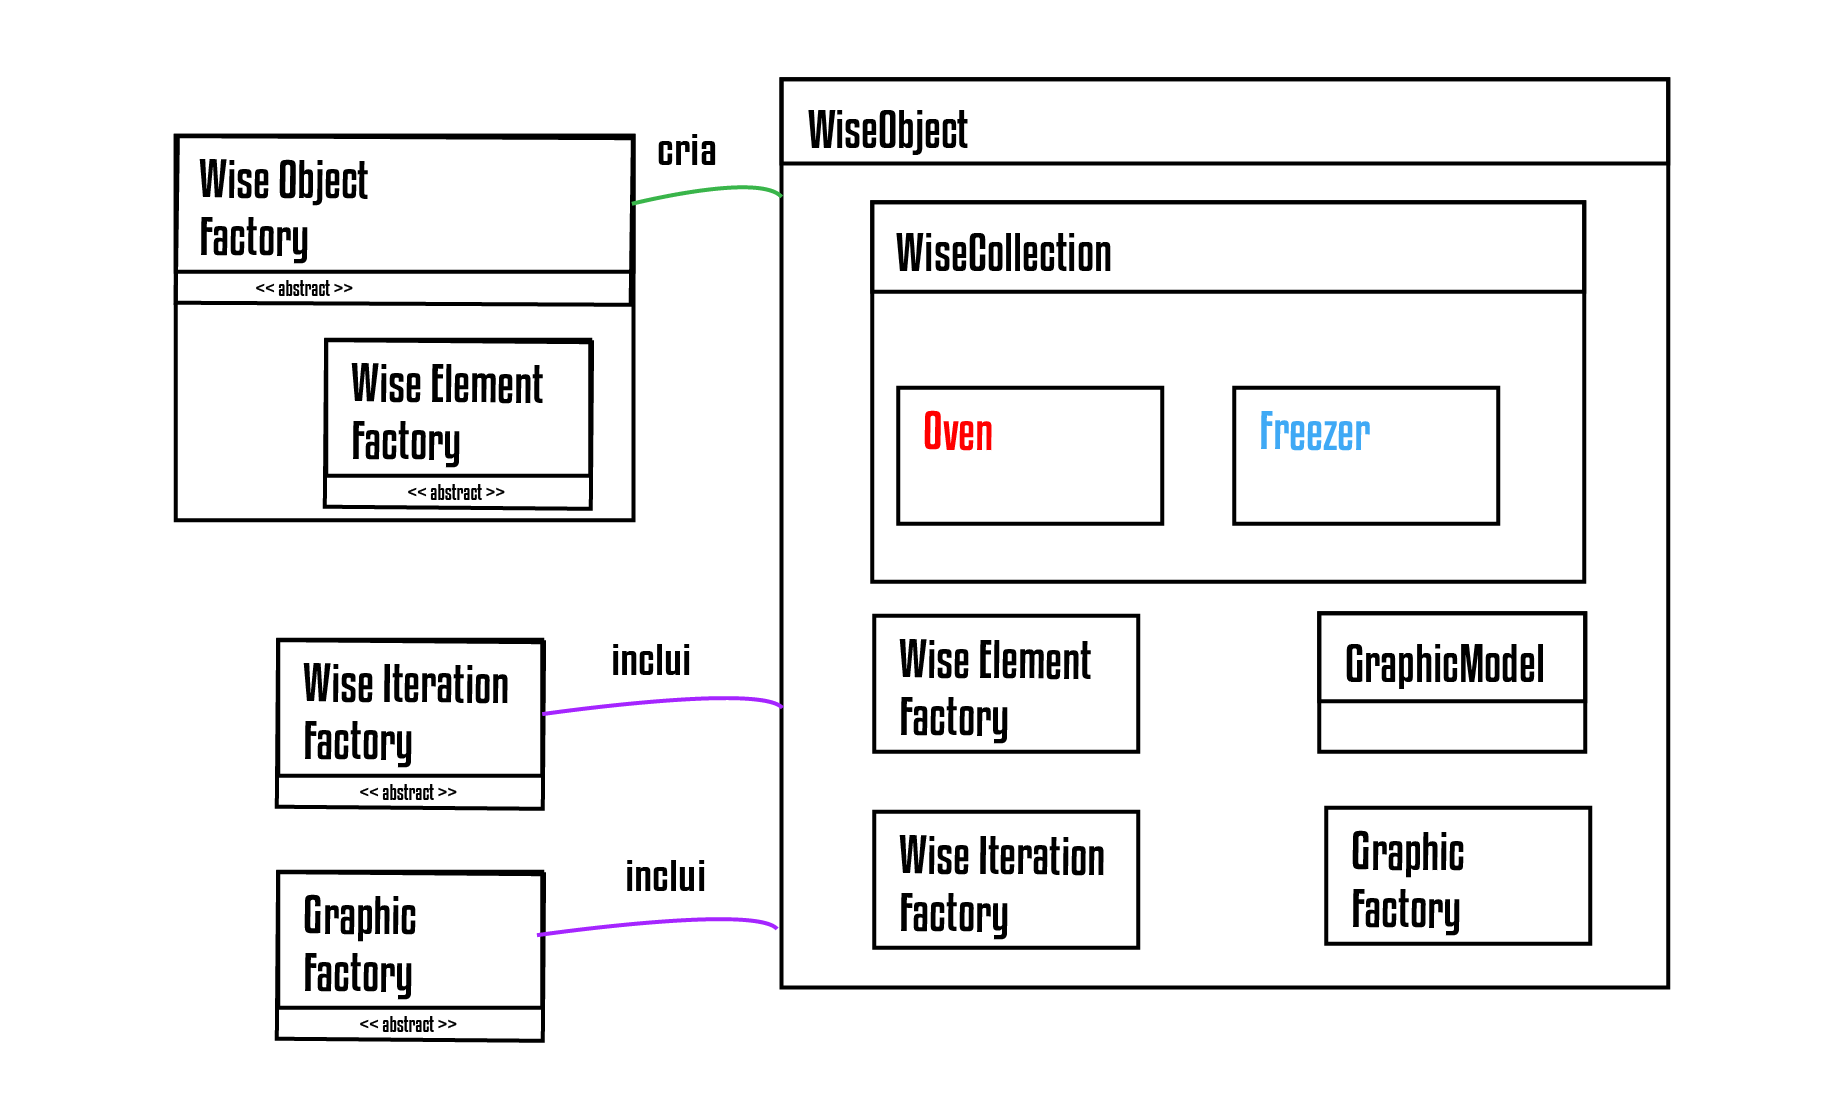
\includegraphics[scale=1]{Figures/WiseObject.png}
	\caption{Objeto inteligente \textit{WiseObject} e todos seu componentes:\textit{WiseObjectFactory}, fábrica responsável pela criação de objetos inteligentes de um predeterminado tipo; \textit{WiseIterationFactory}, fábrica de iteração; \textit{WiseGraphicFactory}, fábrica gráfica; \textit{WiseCollection}, coleção de elementos inteligentes; \textit{GraphicModel}, coleção de objetos gráficos.}
	\label{fig7:wiseobject}
\end{figure}

Através do modelo de classes de um objeto inteligente presente na Figura~\ref{fig7:wiseobject} é possível identificar todos os componentes presentes em um objeto inteligente. Quando se gera um objeto inteligente é incluida a fábrica de criação de elementos inteligentes correspondente, \textit{WiseElementFactory}, que é capaz de criar elementos vazios ou cloná-los. A coleção de elementos inteligentes, \textit{WiseCollection}, contém duas outras estruturas, um forno e um freezer. Estas estruturas são um ponteiro para um elemento obrigatoriamente no estado quente e um lista de objetos frios, respectivamente. O forno apresenta com o elemento que será utilizado durante as iterações, enquanto o freezer é responsável por gerir as estruturas que foram geradas previamente.

Objetos inteligentes também tem seu funcionamento descrito por uma máquina de estados. Diferentemente dos estados de um elemento inteligente os estados de um objeto inteligente não tem relação com os dados armazenados em cache ou com os dados abstratos. Os estados de um objeto inteligente regulam o processo iterativo e de visualização de um objeto inteligente.

\begin{figure}[!htbp]
	\centering
	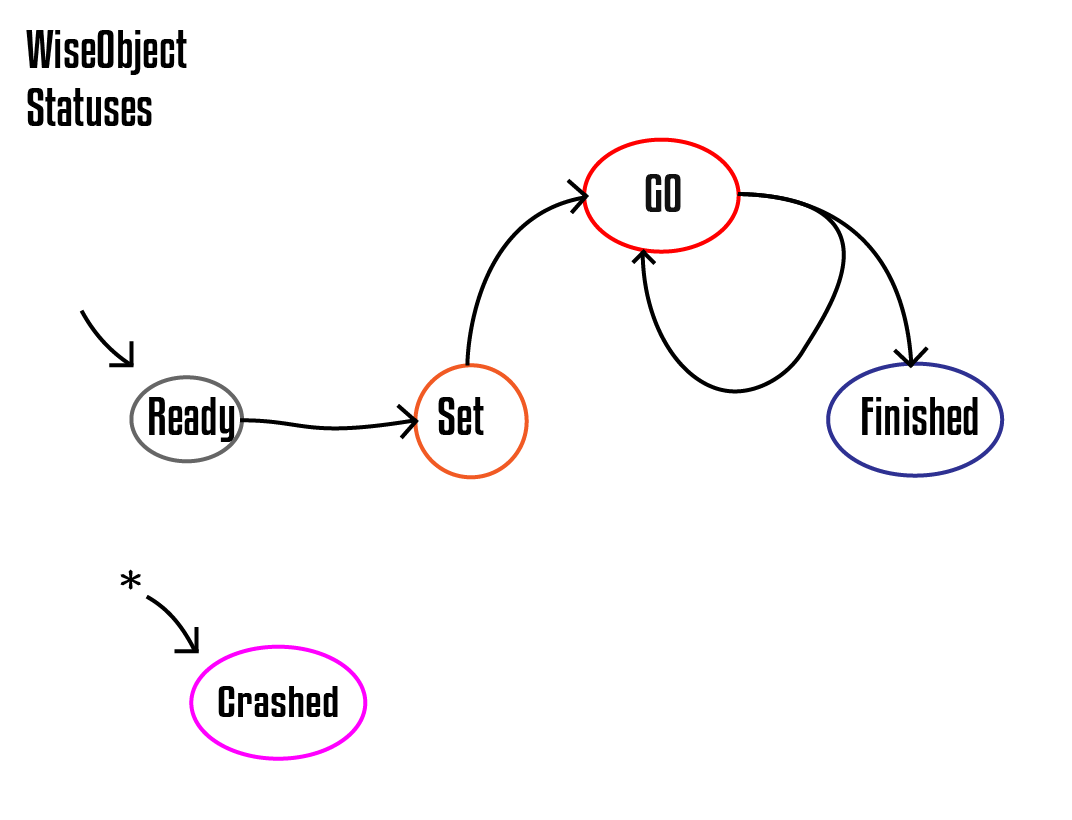
\includegraphics[scale=1]{Figures/WiseObjectStatus.png}
	\caption{Modelo gráfico \textit{GraphicModel}, contém uma coleção de objetos gráficos.}
	\label{fig7:wiseobjectstatuses}
\end{figure}

Diferentemente da troca de estados presente nos elementos inteligentes, aqui a troca se dá por comandos do usuário. Portanto cabe ao usuário indicar as fábricas à serem adicionadas bem como os valores de parâmetros desejados. Para o caso de escoamento pulsátil através de uma árvore arterial é necessário se adicionar a fábrica de iteração correspondente ao algoritmo da seção~\ref{sec:algoritmo} e em seguida definir os parâmetros desejados, como a frequência, a viscosidade e o ângulo de fase. Quando as alterações são concluídas pelo usuário é ele que faz também a mudança de estados.

Inicialmente, um objeto é criado no estado \textit{Ready} com somente dois elementos gráficos e uma fábrica do tipo \textit{WiseElementFactory}. Neste estado é esperada a inclusão das fábricas de iteração e gráficas. Uma vez que elas estejam corretamente acopladas ao objeto inteligente, é possível fazer a troca do estado \textit{Ready} para o estado \textit{Set}. Com a mudança de estado, é adicionado à estrutura \textit{WiseStructure} todos os parâmetros disponibilizados pela fábrica de iteração e, caso tenha sido incluída, fábrica gráfica. Um objeto no estado \textit{Set} indica que o objeto foi corretamente criado, uma fábrica de iteração foi adicionada, possivelmente uma fábrica gráfica também foi adicionada e agora aguarda alterações nestes parâmetros.

Com os parâmetros definidos e as fábricas devidamente acopladas os objeto está pronto para a iteração. O processo iterativo de um objeto inteligente é representado na transição para o estado \textit{Go}. Uma iteração de uma \textit{WiseArteryTree} representa o cálculo dos valores de pressão e fluxo em toda a árvore arterial. Caso algum erro ocorra durante o processamento de dados o objeto se desloca para o estado \textit{Crashed}, assim como elementos inteligentes. É possível também finalizar a execução de um objeto inteligente o enviando para o estado \textit{Finished}, neste estado o objeto não poderá ser iterado novamente. O objeto inteligente também pode ser reiniciado à partir de qualquer estado, o que significa que todas as alterações feitas na estrutura do objeto inteligente serão apagadas. Para que parâmetros da iteração possam ser alterados sem que se perda os dados até então definidos é possivel que um objeto no estado \textit{Go} seja resetado e transite para o estado \textit{Set}.

%--------------------------------------------------------------------------------%
\subsection{Objeto Gráfico}\label{sec:objeto_grafico}

Caso seja configurado, o objeto inteligente pode incluir os componentes de visualização: fábrica gráfica \textit{GraphicFactory} e coleção de objetos gráficos \textit{GraphicModel}. Somente depois de adicionar uma fábrica gráfica à um objeto que a coleção de objetos gráficos é alocada e o primeiro objeto gráfico criado. Objetos gráficos assim como elementos inteligentes são colecionados por outras estruturas. Enquanto a estrutura responsável por elementos inteligentes, \textit{WiseCollection}, é responsável por manter os últimos dados de iteração aquecidos, a estrutura \textit{GraphicModel} mantém o objeto que está sendo exibido por alguma tela e elementos próximos.

\begin{figure}[!htbp]
	\centering
	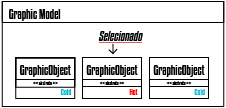
\includegraphics[scale=1]{Figures/GraphicModel.png}
	\caption{Modelo gráfico \textit{GraphicModel}, contém uma coleção de objetos gráficos.}
	\label{fig7:graphicmodel}
\end{figure}

Presente na Figura~\ref{fig7:graphicmodel} estão os componentes que permitem armazenar todos os quadros da animação final ao visualizar algum parâmetro contido na estrutura \textit{WiseStructure}. Quando um objeto \textit{WiseObject} está corretamente configurado com uma instância de fábrica gráfica \textit{GraphicFactory}, seu método iterativo é atrelado à iteração do objeto. Isso permite que o objeto iterado crie um elemento inteligente \textit{WiseElement} e um objeto gráfico \textit{GraphicObject} à cada iteração.

\begin{figure}[!htbp]
	\centering
	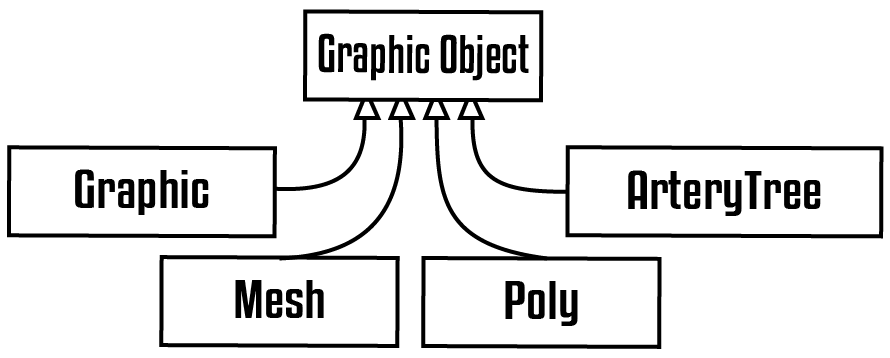
\includegraphics[scale=1]{Figures/GraphicObjects}
	\caption{Tipos de objetos gráficos \textit{GraphicObjects}.}
	\label{fig7:graphicobjects}
\end{figure}


Os objetos gráficos contidos na Figura~\ref{fig7:graphicobjects} de cada tipo se desenha através de um gradiente de cores e formas geométricas padrão, bidimensionais ou tridimensionais. Cada forma geométrica utilizada é representada por elementos gráficos, objeto que implementam a classe abstrata \textit{GraphicElement}. Cada elemento gráfico é atrelado à um valor ou à uma lista de valores, estes valores são utilizados para dar cor aos elementos gráficos. Cada objeto gráfico possui um valor máximo e mínimo que é vinculado ao gradiente cores, com isso as cores representam os valores armazenados em cada elemento.

\begin{figure}[!htbp]
	\centering
	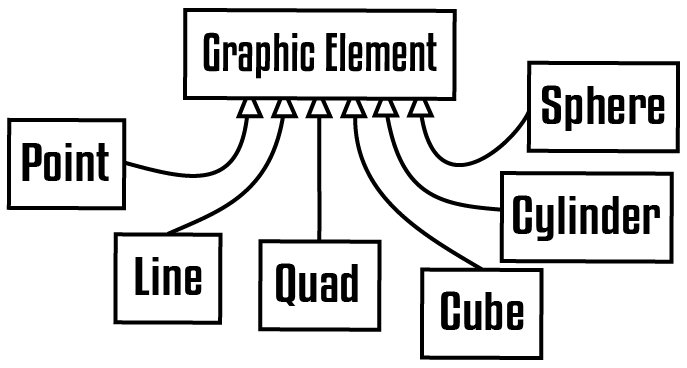
\includegraphics[scale=1]{Figures/GraphicElements}
	\caption{Tipos de elementos gráficos \textit{GraphicElements}. \textit{Point}, um ponto. \textit{Line}, uma linha. \textit{Quad}, um quadrado. \textit{Cube}, um cubo. \textit{Cylinder}, um cilindro. \textit{Sphere}, uma esfera.}
	\label{fig7:graphicelements}
\end{figure}

Os elementos gráficos podem ser utilizados por qualquer tipo de objeto gráfico. A representação geométrica de uma árvore arterial é construída utilizando cilindros e esferas, que representam segmentos de vaso e terminais, respectivamente. Os cilindros receberão uma lista de valores da pressão $P(X) \forall X \in [0,1]$, enquanto as esferas receberão os valores da pressão $P(X)$ quando $X=0$ ou $X=1$, dependendo se é o nó distal($X=1$) ou o nó proximal($X=0$).

%-------------------------------------------------------------------------------------------%
\chapter{RESULTADOS NUMÉRICOS E DISCUSSÕES}

Assim como os objetos inteligentes \textit{WiseObject} têm seus tipos definidos pelo tipo de elemento inteligente que o compõe, o tipo de objeto gráfico segue o tipo de elemento inteligente que representa.
\textcolor{red}{IGOR: já fiz uma primeira revisão deste capítulo e indico em vermelho o que deve fazer para melhorar este capítulo. Tudo que acrescentar ou mudar coloque em azul.}
\textcolor{blue}{XXXXXXXXXXXXX}.
\textcolor{red}{IGOR: não está aparecendo a numeração das Figuras no caption. Algo de errado está acontecendo no modelo que está utilizando.}
\textcolor{red}{IGOR: está errada a citação do trabalho do método de Duan e Zamir (1995), não é a citação que colocou \cite{Duan}.}

Nesta seção, apresentam-se resultados obtidos com a implementação computacional e simulação do modelo matemático de Duan e Zamir~\cite{Duan}. As simulações realizadas aqui tratam da propagação de uma onda harmônica simples ao longo de uma árvore, onde reflexões de onda modificam a amplitude da onda de pressão enquanto ela avança. A escolha de uma onda harmônica simples neste estudo possibilita investigar os efeitos da frequência, fluido viscoso e viscoelasticidade da parede do segmento de vaso.

Considerou-se neste estudo um modelo de árvore arterial canina como ilustrado na Figura~\ref{fig:arvore-canina}. As propriedades dos segmentos foram escolhidas oriundas dos dados de Fung~\cite{Fung} e são descritas na Tabela~\ref{tab1:proprerty}. 

\begin{figure}[!htbp]
	\centering
	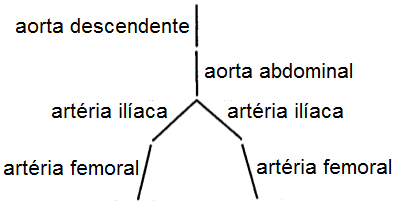
\includegraphics[scale=0.8]{Figures/tree_canine.png}
	\caption{Representação do modelo de árvore arterial canina (figura adaptada de~\cite{Duan}).}
	\label{fig:arvore-canina}
\end{figure}

\begin{table}[!htbp]
	\caption{Propriedades dos segmentos do modelo de árvore arterial~\cite{Duan,Fung}}
	\centering{}
	\begin{tabular}{|c||c|c|c|c|c|}
		\hline 
		Artéria	& Comprimento & Densidade & Viscosidade  & Diâmetro & Módulo de  \\ 
		& ($cm$) & $\rho$ ($g/cm^3$) & $\mu_0$ ($g/cm s$) & ($cm$) & Young ($dyn/cm^2$) \\ 
		\hline
		\hline 
		Aorta & 25 & $0,960$ & 0,0385 & 1,3 &4,8 $\times 10^6$ \\ 
		Descendente &  & &  & & \\ 
		\hline 
		Aorta & 11 & $1,134$ & 0,0449 & 0,9 & 1,0 $\times 10^7$ \\
		Abdominal &  & &  & &  \\ 
		\hline 
		Ilíaca & 12 & $1,172$ & 0,0472 & 0,6 & 1,0 $\times 10^7$\\ 
		\hline 
		Femoral & 10 & $1,235$ & 0,0494 & 0,4 & 1,0 $\times 10^7$\\ 
		\hline 
	\end{tabular} 
	\label{tab1:proprerty}
\end{table}

Nas simulações aqui realizadas, calculou-se a distribuição de amplitude de pressão ao longo da árvore arterial (Figura~\ref{fig:arvore-canina}). Os resultados foram obtidos para quatro diferentes frequên\-cias e três diferentes cenários de escoamento/segmento: (i) escoamento viscoso em segmento puramente elástico (cenário 1 da Seção~\ref{sec:cenario}), (ii) escoamento invíscido em segmento viscoelástico (cenário 2) e (iii) escoamento viscoso em segmento viscoelástico (cenário 3). 

Os resultados obtidos nas simulações são mostrados nas Figuras~\ref{fig3a:arterial-tree}, \ref{fig3b:arterial-tree}, \ref{fig4a:arterial-tree}, \ref{fig4b:arterial-tree}, \ref{fig5a:arterial-tree} envolvendo a amplitude da pressão ao longo do modelo de árvore arterial. Nestas figuras, o comprimento de cada segmento arterial foi dimensionado para 1,0, de modo que o comprimento adimensional total da árvore é 4,0. O comprimento real é 58 cm. A amplitude da pressão também foi escalada pela pressão de entrada $P_o$, e os resultados finais são portanto mostrados em termos de amplitude de pressão adimensional $|P|$ versus a distância adimensional $X$ do início da árvore.

Nas Figuras~\ref{fig3a:arterial-tree} e \ref{fig3b:arterial-tree}, o efeito da viscosidade do fluido é examinado separadamente conside\-ran\-do-se o escoamento em segmentos puramente elásticos com quatro valores diferentes de viscosidade do fluido, ou seja, $\mu = 0$; $0,5 \mu_0$; $1,0 \mu_0$ e $1,5 \mu_0$, onde $\mu_0$ é o valor base da viscosidade da Tabela~\ref{tab1:proprerty}. Observa-se que o efeito da viscosidade do fluido é reduzir o aumento global na amplitude da onda de pressão causada pelas reflexões das ondas à medida que a onda se desloca na direção à jusante. Além disso, modera os picos locais na distribuição de pressão.

\begin{figure}[!htbp]
	\centering
	(a) \\
		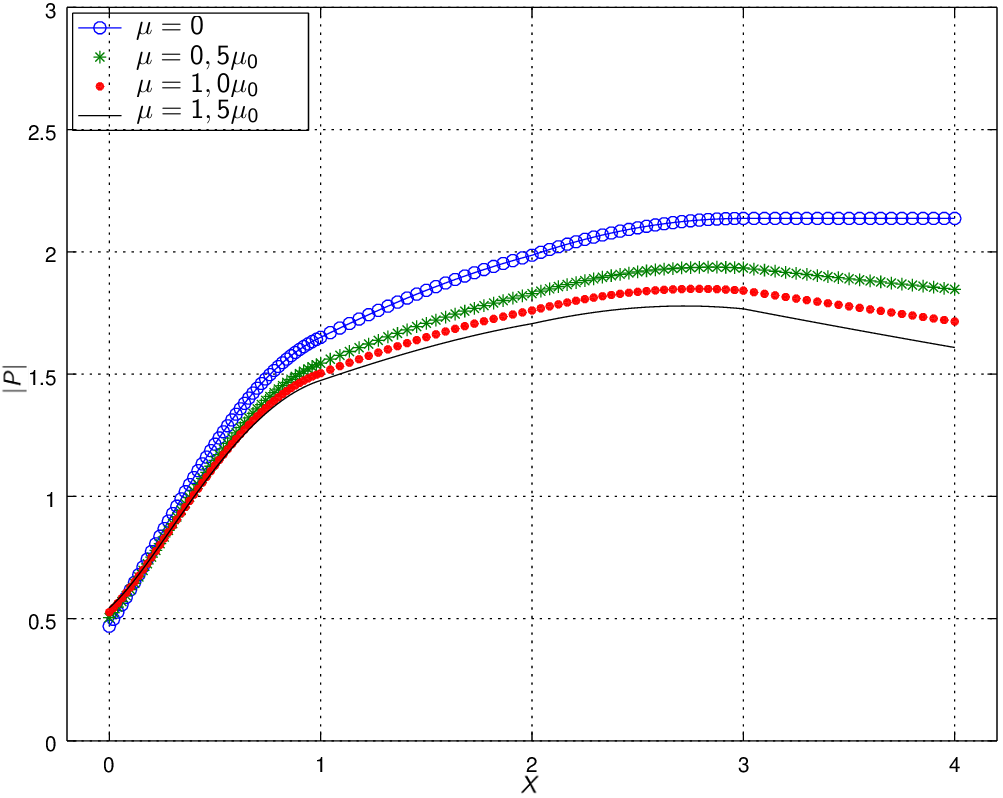
\includegraphics[scale=0.7]{figure3-result-new/fig3_P_f3_65_visc_new2.png}\\
	(b)\\
	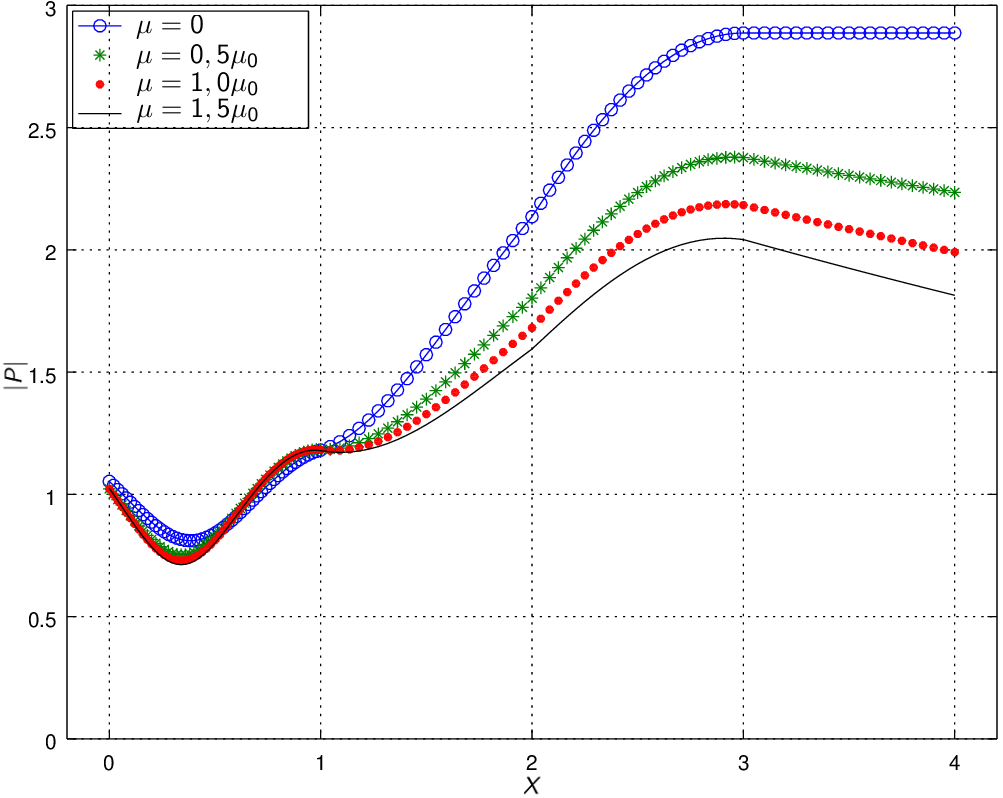
\includegraphics[scale=0.7]{figure3-result-new/fig3_P_f7_30_visc_new2.png}\\
	\caption{Amplitude da pressão $|P|$ ao longo da árvore arterial considerando diferentes viscosidade do fluido $\mu$ e frequências: (a) $f$ = 3,65 Hz, (b)  $f$ = 7,30 Hz. }
	\label{fig3a:arterial-tree}%
\end{figure}

\begin{figure}[!htbp]
	\centering
	(a) $f$ = 10,95 Hz\\
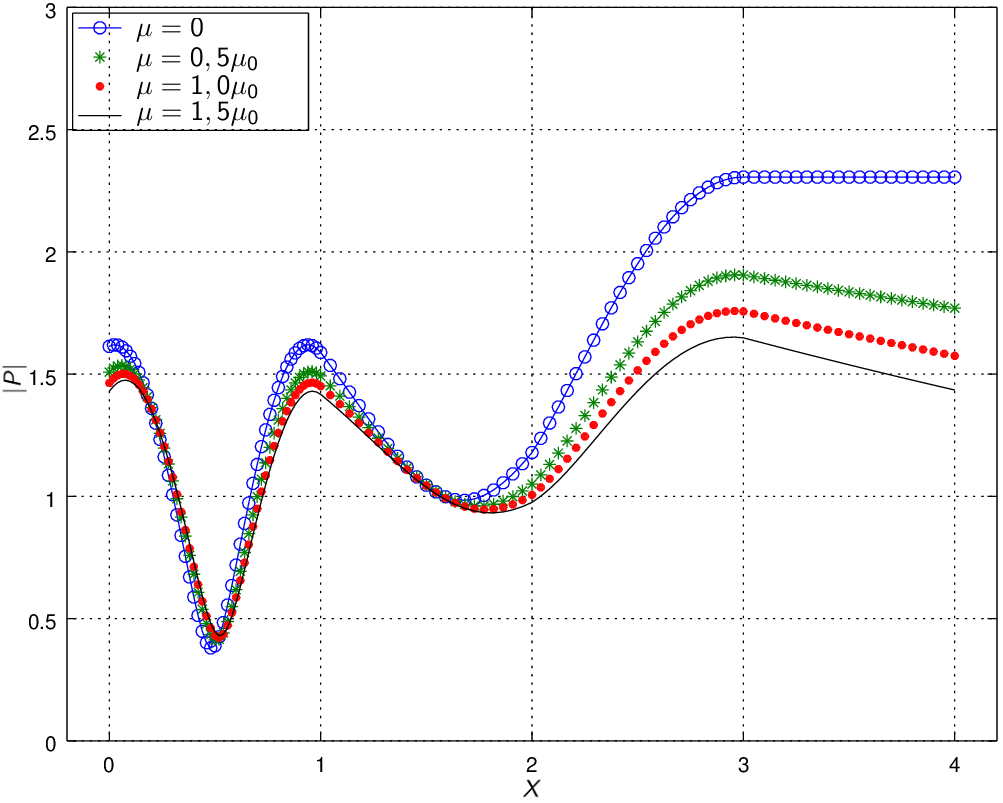
\includegraphics[scale=0.7]{figure3-result-new/fig3_P_f10_95_visc_new2.png}\\
	(b) $f$ = 14,60 Hz\\
	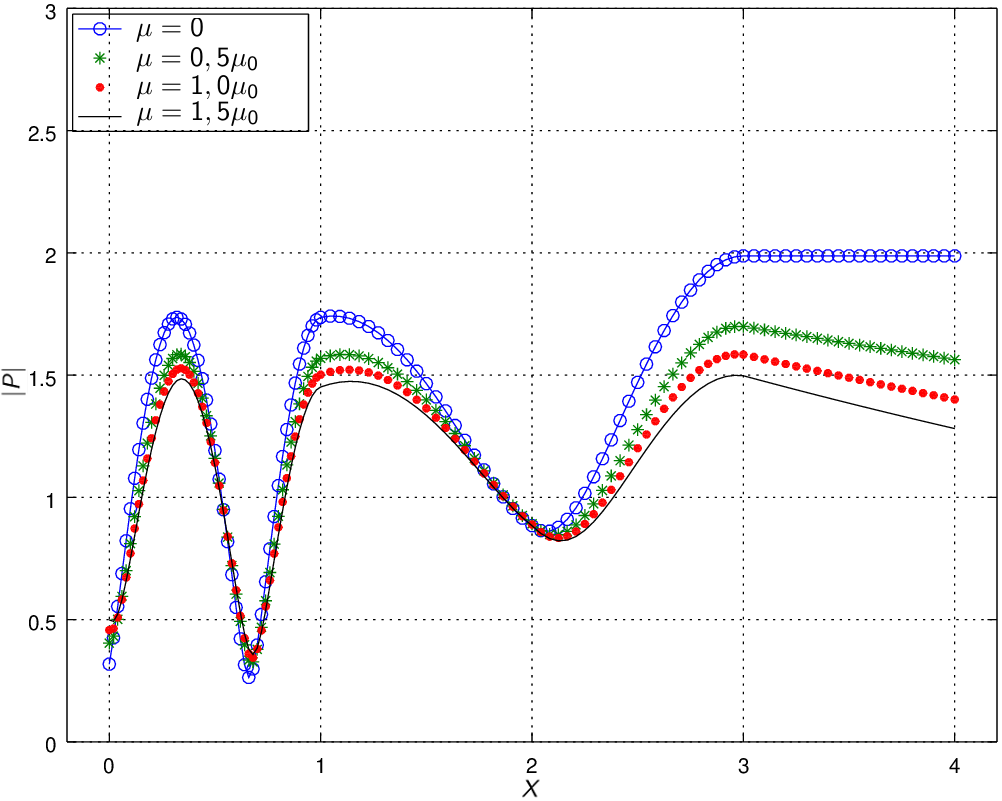
\includegraphics[scale=0.7]{figure3-result-new/fig3_P_f14_60_visc_new2.png}\\
	\caption{Amplitude da pressão $|P|$ ao longo da árvore arterial considerando diferentes viscosidade do fluido $\mu$ e frequências: (a) $f$ = 10,95 Hz, (b)  $f$ = 14,60 Hz. }
	\label{fig3b:arterial-tree}%
\end{figure}

Nas Figuras~\ref{fig4a:arterial-tree}, \ref{fig4b:arterial-tree}, o efeito da viscoelasticidade da parede do segmento de vaso é considerado separadamente considerando-se o escoamento invíscido e tomando-se quatro valores diferentes da viscoelasticidade da parede do segmento. O modelo viscoelástico proposto utilizado para fins destes cálculos é apresentado no cenário 2 da Seção~\ref{sec:cenario}, no qual a viscoelasticidade da parede do vaso é representada por um módulo de Young complexo. Estas figuras mostram os resultados para $\phi_0$ = $0^o$, $4^o$, $8^o$ e $12^o$. Quando $\phi_0$ = $0^o$ tem-se um valor representando uma parede puramente elástica e para $\phi_0> 0$ tem-se a representação da viscoelasticidade. Nota-se a partir destas figuras que o efeito da viscoelasticidade, como o da viscosidade do fluido, é amortecer o aumento global da amplitude da onda de pressão causada pelas reflexões das ondas à medida que a onda se desloca na direção à jusante, bem como moderar os picos locais na distribuição de pressão. 

\begin{figure}[!htbp]
	\centering
	(a) \\
	\includegraphics[scale=0.7]{figure4-result-new/Fig4_P_f3_65_visco_new2.png}\\
	(b)\\
	\includegraphics[scale=0.7]{figure4-result-new/Fig4_P_f7_30_visco_new2.png}\\
	\caption{Amplitude da pressão $|P|$ ao longo da árvore arterial considerando diferentes valores de viscoelasticidade $\phi_0$ e frequências: (a) $f$ = 3,65 Hz, (b)  $f$ = 7,30 Hz. }
	\label{fig4a:arterial-tree}%
\end{figure}

\begin{figure}[!htbp]
	\centering
	(a) $f$ = 10,95 Hz\\
	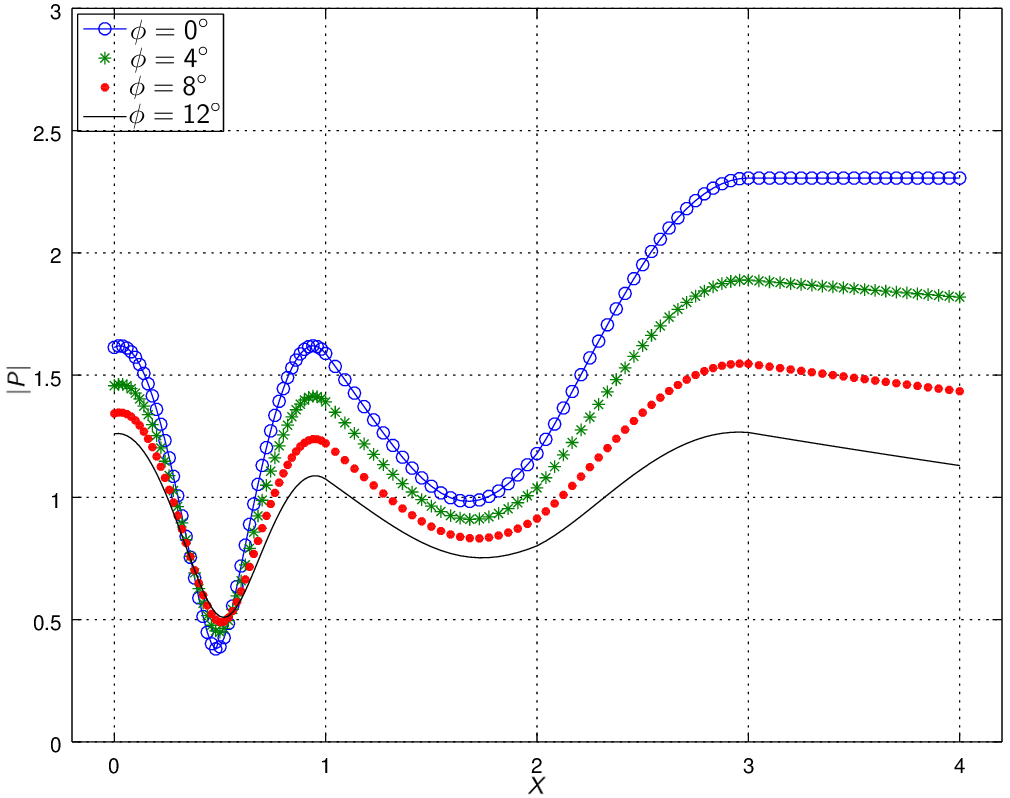
\includegraphics[scale=0.7]{figure4-result-new/fig4_P_f10_95_visco_new2.png}\\
	(b) $f$ = 14,60 Hz\\
	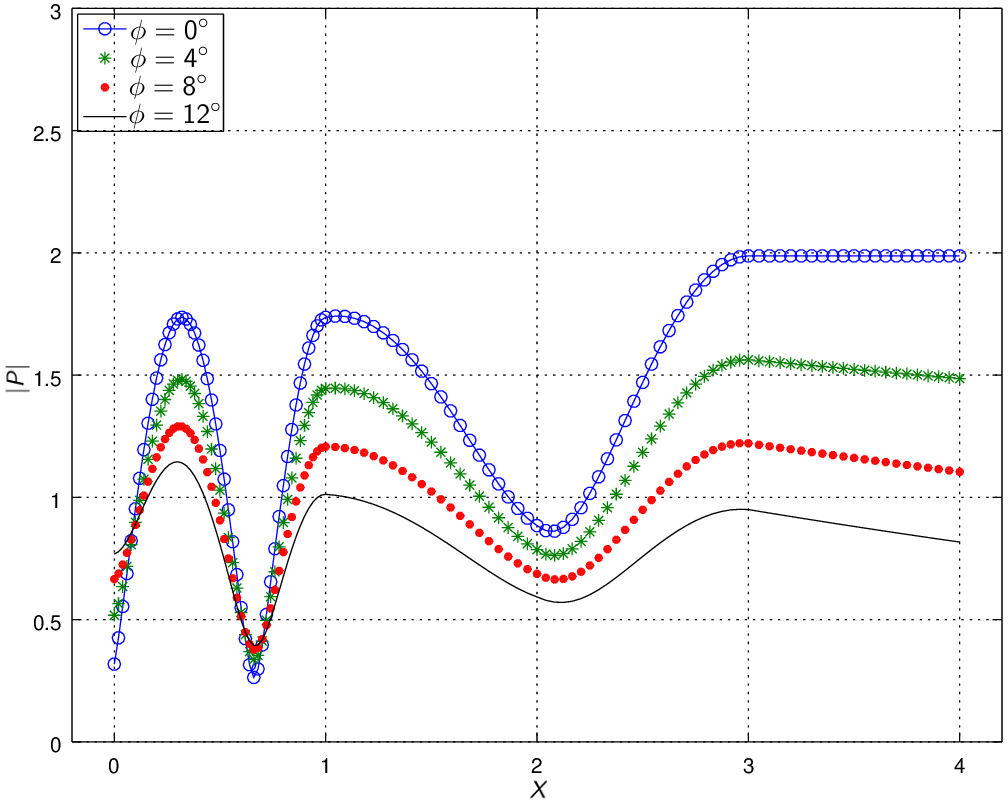
\includegraphics[scale=0.7]{figure4-result-new/fig4_P_f14_60_visco_new2.png}\\
	\caption{Amplitude da pressão $|P|$ ao longo da árvore arterial considerando diferentes valores de viscoelasticidade $\phi_0$ e frequências: (a) $f$ = 10,95 Hz, (b) $f$ = 14,60 Hz.}
	\label{fig4b:arterial-tree}%
\end{figure}

A Figura \ref{fig:impedance1} apresenta o comportamento da impedância de entrada $|Z|$ em função da frequência $f$, que está coerente com dados experimentais ~\cite{Nichols2011} da aorta. Na Figura \ref{fig:impedance1}a, nota-se que, quando se considera a viscosidade ($\mu \neq 0$) na simulação do método, isso afeta a impedância de entrada para frequências que se aproximam de 0 Hz e atenua o pico que surge na curva entre 10 Hz e 12,5 Hz. Além disso, neste intervalo de frequência, observa-se o aparecimento do pico mencionado em uma frequência ligeiramente menor com o aumento de $mu$.

No tocante ao impacto da viscoelasticidade da parede na impedância de entrada, o aumento do parâmetro $\phi$ reduz o pico que aparece na curva de impedância entre 10 Hz e 12,5 Hz como pode ser visto na Figura \ref{fig:impedance1}b. Diferente da Figura \ref{fig:impedance1}a, o pico destacado surge na mesma frequência independente do $\phi$.

\begin{figure}[!htbp]
	\centering
	(a) \\
	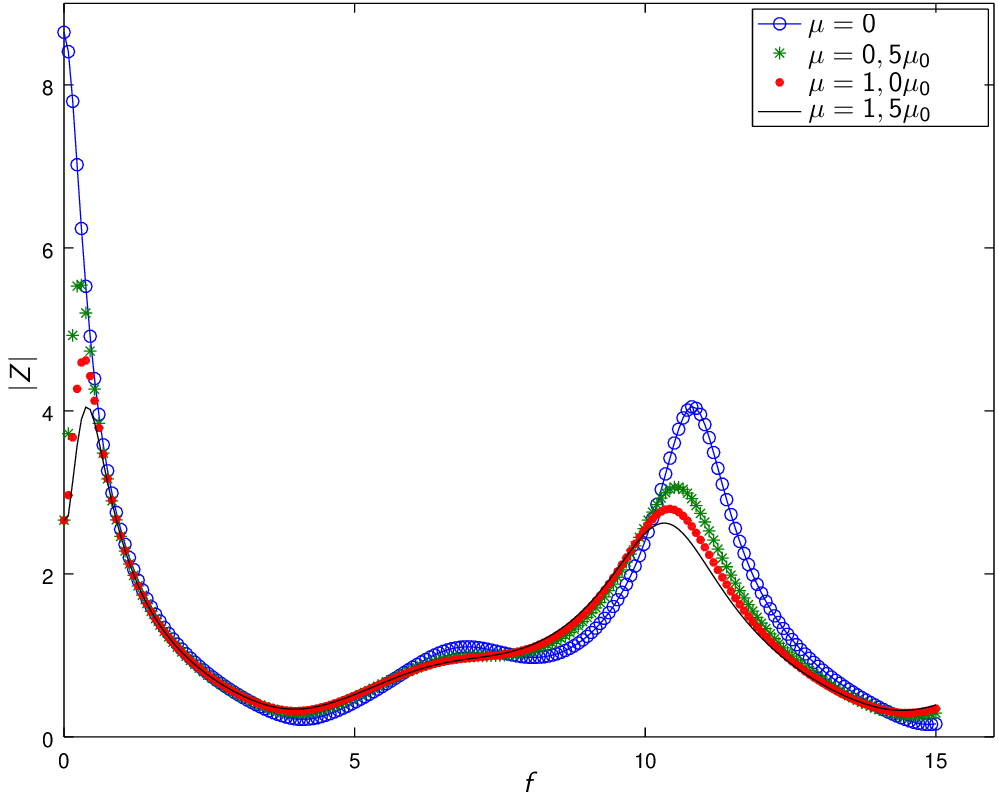
\includegraphics[scale=0.7]{figure-result-impedance/fig_viscosity_impedance_new.png}\\
		(b) \\
	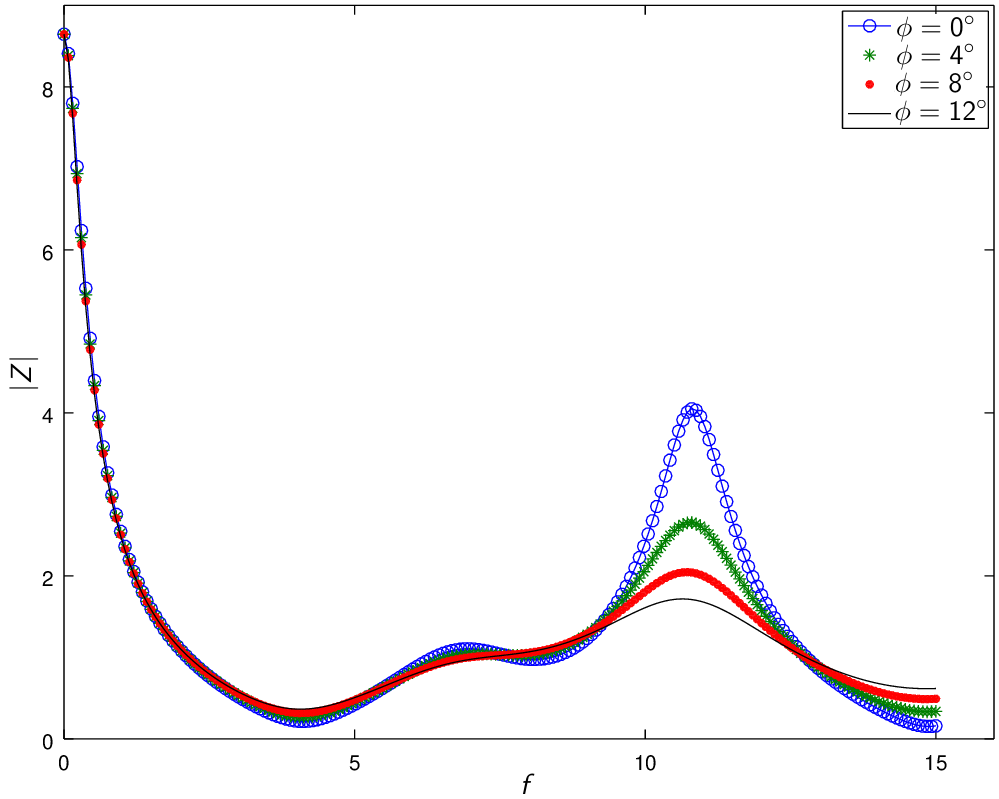
\includegraphics[scale=0.7]{figure-result-impedance/fig_viscoelasticity_impedance_new.png}
	\caption{Amplitude da impedância de entrada $|Z|$ em função da frequência $f$: (a) efeito da viscosidade (b) impacto da viscoelasticidade.}
	\label{fig:impedance1}%
\end{figure}

%\newpage
Os efeitos combinados da viscosidade do fluido e viscoelasticidade da parede do vaso na amplitude de pressão $P$ e impedância de entrada $Z$ são mostrados nas Figuras \ref{fig5a:arterial-tree} e \ref{fig5b:arterial-tree}. Os valores $\mu = 1,0 \mu_0$ e $\phi_0 = 8^o$ foram utilizados para este propósito, para serem comparados com os mesmos valores dos resultados anteriores. A observação mais importante a ser feita é que os dois efeitos, quando combinados, não se somam. Por outro lado, combinam-se de uma maneira não linear que não é prontamente previsível.

\begin{figure}[!htbp]
	\centering
	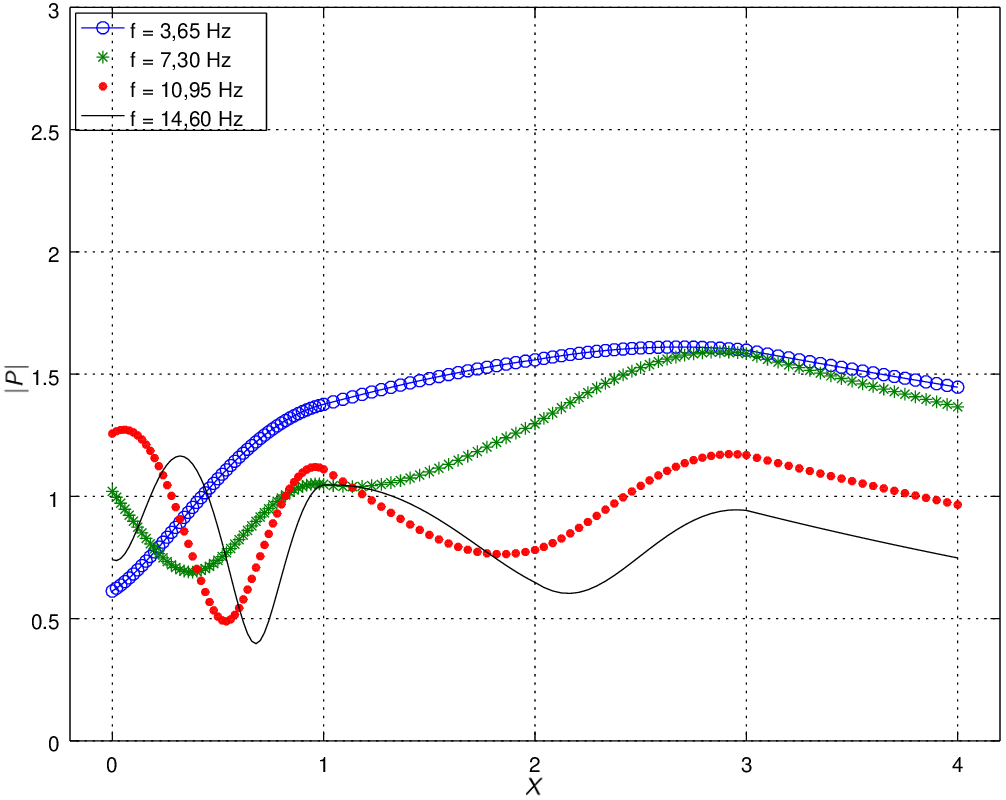
\includegraphics[scale=0.7]{figure5-result-new/Fig5_P_visc1_phi8_new2.png}
	\caption{Amplitude da pressão $|P|$ ao longo da árvore arterial $X$ considerando viscosidade $\mu = 1,0 \mu_0$, viscoelasticidade $\phi_0 = 8^{\circ}$.}
	\label{fig5a:arterial-tree}%
\end{figure}

\begin{figure}[!htbp]
	\centering
	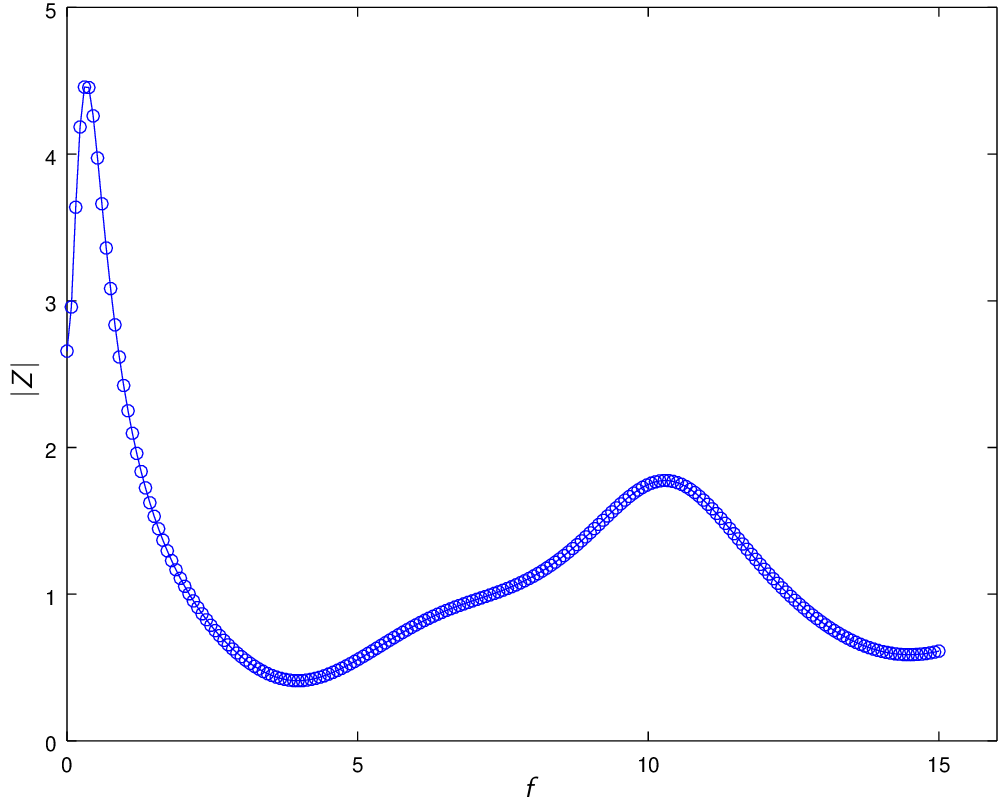
\includegraphics[scale=0.7]{figure-result-impedance/fig_viscosidade1_viscoelasticity8_impedance_new.png}
	\caption{Impedância de entrada $|Z|$ em função da frequência $f$ considerando viscosidade $\mu = 1,0 \mu_0$, viscoelasticidade $\phi_0 = 8^{\circ}$.}
	\label{fig5b:arterial-tree}%
\end{figure}

%-----------------------------------------------------------------------------------------%
\chapter{CONCLUSÕES E TRABALHOS FUTUROS}
\textcolor{red}{IGOR: já fiz uma primeira revisão deste capítulo e indico em vermelho o que deve fazer para melhorar este capítulo. Tudo que acrescentar ou mudar coloque em azul.}
\textcolor{blue}{XXXXXXXXXXXXX}.

Em relação a hemodinâmica, os resultados obtidos neste trabalho estão de acordo com aqueles obtidos por Duan e Zamir \cite{Duan} considerando a propagação de uma onda harmônica simples nos três cenários abordados nas simulações. 

Em destaque, visando contribuir na investigação do método desenvolvido por por Duan e Zamir, curvas de impedância de entrada do modelo de árvore canina aqui considerada foram apresentadas. Estas curvas apresentam comportamento que pode ser observado em dados experimentais.

A realização deste trabalho resultou no desenvolvimento de uma nova ferramenta computacional descrita no Capítulo~\ref{sec:modelagem}, que permite a simulação de escoamento sanguíneo pulsátil em modelos de árvores arteriais no contexto de Duan e Zamir. 

\textcolor{red}{IGOR: escreva um parágrafo destacando propriedades/características e potencialidades da sua ferramenta computacional. Talvez você poderá recuperar ou utilizar algo do parágrafo abaixo.}

\textcolor{red}{A ferramenta simula e analisa modelos de árvores arteriais. Ela pode ser utilizada nos sistemas Operacionais: Windows e o Ubuntu (Unix). Os modelos podem ter sua análise e gráficos gerados automaticamente através dos comandos da ferramenta computacional. O código possibilita o processamento concorrente de diversos modelos em um mesmo ambiente. Cada uma destas contribuições resultou numa ferramenta robusta,  ferramenta esta que além de analisar corretamente as variações de fluxo e pressão através de um modelo de árvore arterial, possibilita que as simulações sejam facilmente ajustadas e analisadas, com ou sem interface gráfica.}

\textcolor{red}{IGOR: o parágrafo acima descreve a ferramenta descrita no Capítulo 3? Este parágrafo representa a descrição da ferramenta.}

Como trabalhos futuros, destacam-se:
\begin{itemize}
    \item Analisar hemodinamicamente modelos de árvores gerados no contexto do método CCO (\emph{Constrained Constructive Optimization}) \cite{Karch1999,Queiroz2013,Queiroz2015,Brito2017};
    \item Investigar a influência da escolha parâmetros na resposta do método, tais como: módulo de Young e espessura do vaso;
    \item \textcolor{red} {IGOR: descreva algo que poderia ser interessante agregar na ferramenta, pode ser mais de uma coisa (coloque em item)}.
\end{itemize}

\bibliographystyle{abntex2-alf}
\bibliography{referencias}

\end{document}
